\documentclass[11pt]{article}

% Default margins are too wide all the way around. I reset them here

\usepackage[a4paper,
			twoside,
			left=1.5in,
			right=1.0in,
			textheight=9in, 
			headheight=14pt]{geometry}
			
\usepackage[utf8]{inputenc}
\usepackage[T1]{fontenc}
\usepackage{lmodern}
\usepackage[danish,english]{babel}
\usepackage{setspace}
\usepackage[pdfborder={0 0 0}]{hyperref}

\usepackage{amsmath}
\usepackage{amsfonts}
\usepackage{amssymb}
\usepackage{graphicx}
\usepackage{csquotes}
\usepackage{appendix}
\usepackage[backend=biber, style=ieee]{biblatex}
\usepackage{algorithm}
\usepackage{algorithmic}
\usepackage{subfigure}
\usepackage{fancyhdr}
\usepackage[labelfont=bf]{caption}
\usepackage{listings}
\usepackage[usenames,dvipsnames,table]{xcolor}

\colorlet{NotLavender}{Lavender!30}
\colorlet{NotGreenYellow}{GreenYellow!30}
\colorlet{NotSkyBlue}{SkyBlue!20}
\colorlet{NotOrange}{Orange!20}
\colorlet{NotRed}{Red!30}
\colorlet{NotGreen}{Green!20}
\colorlet{NotPurple}{Purple!20}

\definecolor{DarkGreen}{rgb}{0.0,0.4,0.0}
\definecolor{highlight}{RGB}{255,251,204}
\renewcommand{\lstlistingname}{Snippet}
\lstset{language=C++, 
		basicstyle=\footnotesize, 
		breaklines=true, 
		breakatwhitespace=false, 
		keywordstyle=\bf\color{Blue},
		firstnumber=1,
		frame=lines,
		numbers=left,
		numbersep=10pt,
		numberstyle=\tiny\color{Gray},
		stepnumber=5,
		stringstyle=\color{Purple},
		commentstyle=\usefont{T1}{pcr}{m}{sl}\color{DarkGreen},
		captionpos=b
}

% \DeclareLanguageMapping{english}{english-apa}
\graphicspath{{images/}}
\addbibresource{bib.bib}


\author{Group Number}
\title{Report Template}

%\includeonly{./chapters/introduction}

\begin{document}

%------------------------------------------------------------------------------
% TITLE
%------------------------------------------------------------------------------
\fancyhf{}
\pagestyle{plain}
\pagenumbering{roman}

\include{./chapters/readersguide}
%!TEX root = ../main.tex

\section*{Glossary} % (fold)
\label{sec:glossary}

Throughout the report you might encounter some terms used to express a certain matter. 
This glossary will try to explain what is meant when these terms are used.

\begin{table}[!h]

\begin{tabular}{p{2in} p{3.4in}}
Auditory display & The use of sound to communicate information from a computer to the user.
\end{tabular}

\begin{tabular}{p{2in} p{3.4in}}
Intuitive & something that is known or understood without proof or evidence.
\end{tabular}

\begin{tabular}{p{2in} p{3.4in}}
Sonification & the use of non-speech audio to convey information.
\end{tabular}

\end{table}


% section glossary (end)

\maketitle
\setcounter{tocdepth}{2}
\tableofcontents

\clearpage
%------------------------------------------------------------------------------
% CONTENT
%------------------------------------------------------------------------------
\setstretch{1.3}
\pagestyle{fancy}
\renewcommand{\sectionmark}[1]{\markboth{#1}{}}
\fancyhead[RE, LO]{Chapter \thesection . \emph{\nouppercase{\leftmark}}}
\fancyhead[RO, LE]{\thepage}
\pagenumbering{arabic}

%!TEX root = ../main.tex

\section{Introduction} % (fold)
\label{sec:introduction}

The weather forecast is a tricky thing. 
Everyone likes to talk about them, everyone have their own opinion about what is important and preferences on how the weather data should be presented to them. 
Some people like for the forecasts to be very detailed, while others prefers them over simplified. 
This is why there are so many weather apps available on the market today and each app presents the forecasts just a bit different from the others. 
Some apps presents the forecasts with a lot of details combined with pretty pictures and animations, while others only presents the most important data and a simplistic animation.

Common for all of them is that they only presents the data visually and not audibly. 
Even on the Tv the focus is visual in form of graphs, radar images and numbers, which a very trustable person in a nice suit interpretes for you.

Presented on their own, weather data do not necessarily make a lot of sense to the individual. 
Unless the individual are aware of, what a wind speed of a meter per second feels like and its effect on other weather conditions. 
However the human being posses an intuition which tells what 30*C feels like and based on that, we make our choice on weather to bring a sweater or not for the day.

Over the course of this report we will explore the areas of sonification and test if it is possible to use sound to create a weather forecast and still use this inborn intuition to understand the message.
We will also test if it is possible to combine visual and sound to get a better understanding of the message of the forecast.

% section introduction (end)



%!TEX root = ../main.tex

\section{Pre-analysis} % (fold)
\label{sec:preanalysis}

For this semester we have chosen the theme \textit{Sonification}.
In researching sonification and audification, it was clear that there are more ways of sonifying data, depending on what kind of data is to be converted, how that information is to be displayed and interacted with. 
Weather information contains many different types of data. 
Some of these could be:
temperature (degrees), sunny or cloudy (either or), wind speed (meters per second), visibility, precipitation (rain/sleet/snow/hail measured in millimeters). 
This means that theoretically a lot of different sonification techniques can be applied to this kind of information. 
Furthermore, we would like to investigate if visually presented weather data can actually be understood, and to which degree, if converted to non-speech sound using sonification. 
Can sonification of some of these data maybe even make the weather information more understandable or relatable? 
For instance, is information about wind or downpour more relatable as sound than numbers? These discussions have led us to the following Initial Problem Statement:


\subsection{Initial Problem Statement} % (fold)
\label{sub:initial_problem_statement}

Is it possible to successfully use sonification to convey relevant information about \newline 
weather conditions as efficiently as visually represented weather applications?

% subsection initial_problem_statement (end)


\subsection{Sonification} % (fold)
\label{sub:sonification}

Sonification is used to convey information through non-speech audio, to get a better understanding of what that is; 
we will explain what kind of communication methods there are and examples of their function (visualization, auditory and sonification).


Visualization is the communication method that we perceive through our eyes e.g. posters, TV, computer, traffic lights, chat systems, pictures, sign language, body language etc. relevant to our IPS, a weather application that shows a weather forecast.


Auditory communication is data that we perceive through our ears just like sonification, but unlike sonification, auditory communication can use speech, which occurs in for instance, radio, TV, computers, telephones, all kinds of equipment and applications that allow you talk with people over distance. 
Sonification only uses non-speech audio to convey information, an example is traffic light junctions all around Denmark. 
When you near a crosswalk you will hear 2 different sounds. 
Both sounds are the same, but they consist of different paces of rhythm. 
One sound (slow) indicates it’s a red light, while the other (fast) indicates it’s safe to walk. 
This helps blind people to know whether to cross or not, and is an example of sonification. 
Sonification is a subset of auditory displays\footnote{\textbf{Auditory display} is the use of sound to communicate information from a computer to the user \cite*{McGookin2004}}. 
There are several uses of sonification, and these will be described in detail below.

% subsection sonification (end)

\subsubsection{Examples of sonification} % (fold)
\label{ssub:examples_of_sonification}
Now that sonification has been defined, let’s delve further into the topic and see what some of the uses for sonification could be. 
A good example to start out with is the use in the medical industry. 
From the beginning of medical school, students are taught to use stethoscopes to listen to tissue, gases and blood pumping through veins \cite*{Barrass1999}. 
Much of the data used for diagnosing a patient’s current status is shown in numbers or graphs, but a graph can be distracting during a demanding task, and it’s possible to synthesise sounds to represent this data instead. 
Medical students were shown to perform better in a setting where some dynamic variables about the patients status were presented with sounds rather than graphs \cite*{Barrass1999}. 
It is also used in MRI scans to identify unhealthy regions of the brain, and listening to such data might help a doctor diagnose an illness that otherwise goes undetected \cite*{Barrass1999}.


Another good example is when blind people traverse in the street; they rely on sounds such as the beeping that presents information about traffic lights. 
There also exists multimedia programs that can make maps and text more accessible to visually impaired people. 
Audiograf is an application that generates sound from part of a diagram selected with finger touch \cite*{Barrass1999}. 
Other programs exist such as Mercator, which makes it easier for a blind person to use graphical computer interfaces, by mapping navigation and buttons into auditory cues. Some web browsers have also been enhanced in a similar way, by using sonifications to present download times, layout, hyperlinks and more\cite*{Barrass1999}.


It is stated that gadgets and applications for the visually impaired using sonification have been mined thoroughly \cite*{Girvin2005}, but scientific alternatives also exist. An example of this is the ULTRA (Universal Laboratory Training and Research Aid), which is a device for blind science students created by David Lunney and Robert Morrison. 
ULTRA can be interfaced to give speech and present readouts from laboratory equipment such as pH probes and resistance thermometers \cite*{Girvin2005}.

\begin{figure}[!htbp]
    \centering
    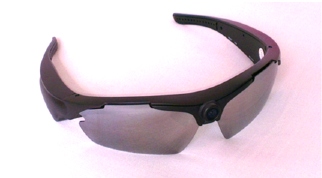
\includegraphics[width=0.95\textwidth]{images/Sonification1.png}
    \caption{vOICe device.}
    \label{fig:sonification1}
\end{figure}

There have also been attempts to create location devices as a replacement for guide dogs.
For example, Dr. Leslie Kay’s “Sonic Torch”, a device using traditional sonar technology, which uses a bat-like frequency sweep to return detailed textural information \cite*{Girvin2005}.
Another attempt at a location device is created by Dr. Peter Meijer and is called vOICe. 
This works by taking the input from a digital camera, either a mounted one or the camera from a cellphone, and using software to sweep the image with a vertical scan line. 
It then sonifies features in the scan by representing vertical position as pitch, horizontal position as time, and brightness by increasing or decreasing volume \cite*{Girvin2005}. 
An interesting result that came from using this device was that a user reported experiences of seeing depth in different places throughout her house. On Dr. Meijer website \url{www.seeingwithsound.com}, a demo of vOICe made in Java can be found. 
On here the application is mentioned as “Augmented Reality for the Totally Blind”. 
Figure~\ref{fig:sonification1} shows an example of how a vOICe device can look. 
The camera in the center is what captures the mage then processed as previously mentioned.
As a last example regarding blind users, Joshua Miele of the Smith Kettlewell Eye Research Institute in San Francisco has written braille support for MATLAB and the sonification toolbox for blind engineers and scientists~\cite*{Girvin2005}. 

% subsubsection examples_of_sonification (end)


\subsubsection{Sonification Techniques} % (fold)
\label{ssub:sonification_techniques}

One way of defining sonifications is describing them according to their sonification techniques.

\begin{enumerate}
    \item Event-based
    \item Model-based
    \item Continuous
\end{enumerate}

The appeal of de Campo’s(XX) approach is that it allows for blurry boundaries between the categories and offers guidance for choosing a sonification technique.


\subsubsection*{Interactivity} % (fold)
\label{ssub:interactivity}

One of the elements to consider when discussing sonification techniques is the interactivity available (or unavailable) to the user of an auditory display. 
Interactivity with auditory displays ranges from completely non-interactive to completely user initiated. 
Non-interactive sonification is often referred to as “concert mode”. 
Instances where the user is able to change and/or choose parameters of the display, has been referred to as “query based” or “conservation mode”. 
User input may also be the driving factor of the presentation of the sound. 

\begin{quote}
``For most sonifications to be useful there must at least be some sort of interactivity, even if it is just play/pause or replay of a certain sound.'' \cite*{Hermann2011}
\end{quote}

% subsubsection interactivity (end)


\subsubsection*{Parameter mapping (event-based sonification)} % (fold)
\label{ssub:parameter_mapping_event_based_sonification_}

``Parameter mapping represents changes in some data dimension with changes in an acoustic dimension to produce a sonification'' \cite*{Hermann2011}.
Sound has many changeable dimension such as frequency, amplitude, phase etc. 
The dimensionality of these data must however be constrained such that a perceivable display is feasible. 
The data changes may be discrete or qualitative. 
For instance, and alarm may be triggered by a discrete on or off threshold, or parameter mapping can be a series of discrete data which makes it seem more continuous. 
These event-based techniques have a passive mode of interaction. 
Some event-based sonifications are brief and offer limited opportunity for user input. 

% subsubsection parameter_mapping_event_based_sonification_ (end)


\subsubsection*{Model-based sonification} % (fold)
\label{ssub:model_based_sonification}

The model-based approach is different from the event-based approaches in that instead of mapping data parameters to sound parameters, the developer builds a virtual model whose sonic responses to user input is derived from data. 
A model is a virtual instrument with which the user can interact with. 
The user input drives the sonification. 
The user learns to understand the structure based on the sonic feedback of the user’s input. 
These types of sonification usually involves large numbers of data points and a high data dimensionality.

% subsubsection model_based_sonification (end)


\subsubsection*{Audification (continues sonification)} % (fold)
\label{ssub:audification_continues_sonification_}

Audification is a direct form of sonification where waveforms of periodic data are directly translated into sound. 
For instance, a Geiger counter gives the user constant sonic feedback of the radiation level by translating data of radiation level into sound.

% subsubsection audification_continues_sonification_ (end)

% subsubsection sonification_techniques (end)


\subsection{Weather Data} % (fold)
\label{sub:weather_data}

Now that we have an overview of what sonification is, we can investigate what weather information is and what types of weather information is usually decided as being relevant to the user.


\subsubsection{What is weather Data?} % (fold)
\label{ssub:what_is_weather_data_}
Weather data is derived from weather forecasting. 
Weather forecasting attempts to predict the state of the atmosphere for a given location, using science and technology.

\begin{quote}
``Weather forecasts are made by collecting quantitative data about the current state of the atmosphere on a given place and using scientific understanding of atmospheric processes to project how the atmosphere will evolve on that place.'' \cite*{Wiki2014-1}
\end{quote}

Weather forecasts are used for a variety of different purposes. 
For instance, weather warnings used to alert societies of dangerous weather, precipitation and temperature is important in agriculture, road surface conditions is important to traffic etc.
On everyday basis, weather forecasts are used to determine what clothes to wear, traffic and travel time, and to plan outdoor activities on a given day. 
Nowadays weather forecasting relies on computer-based models that take many different atmospheric factors into account. 
There is a big range of different weather data, some of these are:

\begin{itemize}
     \item \textbf{Temperature/Dewpoint} - Current air temperature 2 meters above terrain.
     \item \textbf{Wind speed} - Average wind speed over 10 minutes, 10 meters above terrain.
     \item \textbf{Wind direction} - Average wind direction in degrees.
     \item \textbf{Air pressure} - Pressure at sea level measured i hPa (Hectopascal).
     \item \textbf{Humidity} - Current relative humidity measured 2 meters above terrain, measured in percent.
     \item \textbf{Precipitation} - Rain/sleet/snow/hail over the past ten minutes measured in mm.
     \item \textbf{Sun hours} - Hours with sun in a day.
     \item \textbf{Pollen Forecast} - The potency of the pollen. 
     \item \textbf{Sunrise / sunset} - Time of day where the sun rises and sets.
     \item \textbf{Cloud cover}
     \item \textbf{Wind chill} - The winds effect on air temperature.
     \item \textbf{Visibility} - How far can you see with clear line of sight.
     \item \textbf{UV-index} - Intensity of UV radiation.
     \item \textbf{Fronts} 
     \item \textbf{Source Regions} - Where the air is coming from.
     \item \textbf{Drought} - Risk of drought. Presented as a scale.
 \end{itemize}

These are just some of the weather data available in modern weather forecasting. 
Not all of these are necessarily relevant to one single individual, and weather forecasts meant for the general public (not fields of work/study that require very specific weather data) limit the amount and range of weather data presented for the sake of clarity and time (both to present the information but also the time required by the individual to get the information relevant to most). 
Below are some examples of what types of weather data have been chosen to be presented to the viewer on certain weather websites and popularly used weather applications.

% subsubsection what_is_weather_data_ (end)


\subsubsection*{DMI.dk (Danish Meteorological Institute)} % (fold)
\label{ssub:dmi_dk_danish_meteorological_institute_}

DMI.dk is the website of the danish national meteorological institute. 
It is arguably the most well known website containing weather information, in Denmark. 
The website contains a huge amount of weather data, which makes it a bit difficult to navigate and find even the basic weather forecast of the day/week. 
Navigating through the site you will however be able to find information about the atmosphere in a given region such as:
radar images of precipitation, satellite images, lightning probability, ozone measurements, snow depths, and drought indexes, in addition to to the more standard weather information such as wind speed, temperature, precipitation (represented as a graph) and so on. 

\begin{figure}[!htbp]
     \centering
     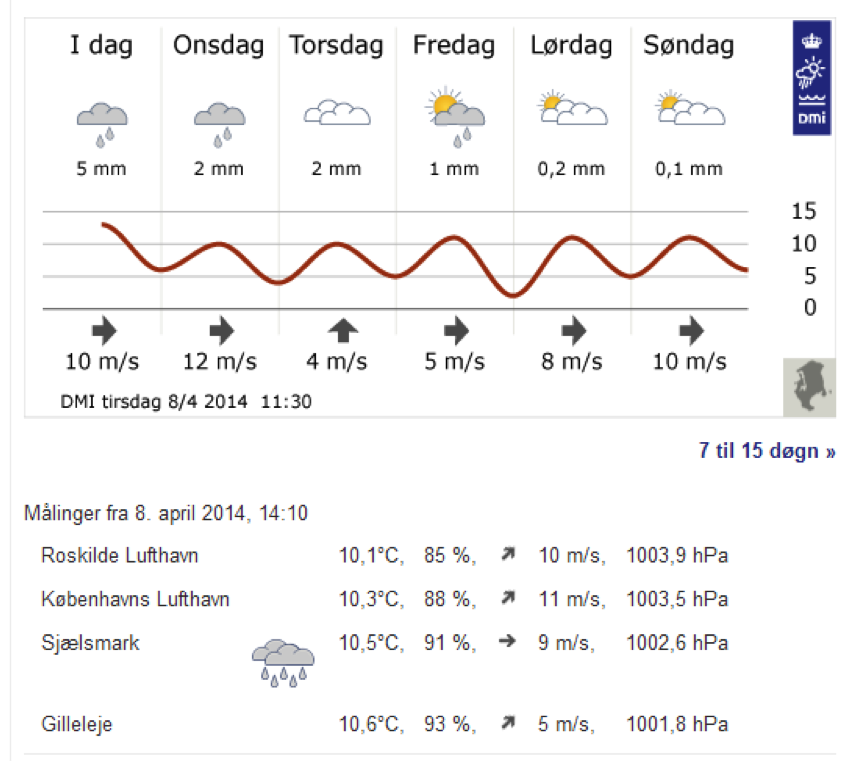
\includegraphics[width=.75\textwidth]{images/Dmi1.png}
     \caption{7-day forecast from DMI.dk}
     \label{fig:dmi1}
 \end{figure}

However, in order to give a shorter, but more clear forecast, you have the option to get a graphically presented 7-day prognosis (Figure~\ref{fig:dmi1}).


This is the basic weather data chosen to be relevant to the general public, and thus this is the prognosis we will be comparing with the other forecasts. 
The 7-day prognosis on DMI.dk contains information about:

\begin{itemize}
    \item Precipitation
    \item Cloud cover
    \item Temperature
    \item Wind speed
    \item Wind direction
\end{itemize}

Additionally, information measured at a certain point of the current day at predetermined locations (April 8, 2014 - 14:10) is presented:

\begin{itemize}
    \item Temperature
    \item Visibility
    \item Wind direction
    \item Wind speed
    \item Atmospheric pressure
\end{itemize}

There is also a summary of the current day’s forecast.

% subsubsection dmi_dk_danish_meteorological_institute_ (end)


\subsubsection*{TV2 Vejret App} % (fold)
\label{ssub:tv2_vejret_app}

TV2 Vejret is a weather app developed by danish TV channel TV2 for iOS and Android. 
The app pulls weather data directly from the TV2 weather center, where the TV stations meteorologists work on predicting the weather for the TV2 news, website and the weather app.


The app finds the phones current location via GPS and retrieves weather information about that area. 
In terms of relevant data, the app gives a fairly limited amount of information (at least compared to DMI.dk), but covers the basic data such as:

\begin{itemize}
    \item Precipitation
    \item Wind speed
    \item Wind direction
    \item Sun up/down
    \item UV index
    \item Cloud cover
    \item Temperature
\end{itemize} 

From figure~\ref{fig:tv21} it is apparent that most of the information is only presented for the current time of day. 
Prognosis for the next 14 days is limited to:

\begin{itemize}
    \item Cloud cover
    \item Temperature
    \item Precipitation
    \item Wind speed
    \item Wind direction
\end{itemize}

\begin{figure}[!htbp]
    \centering
    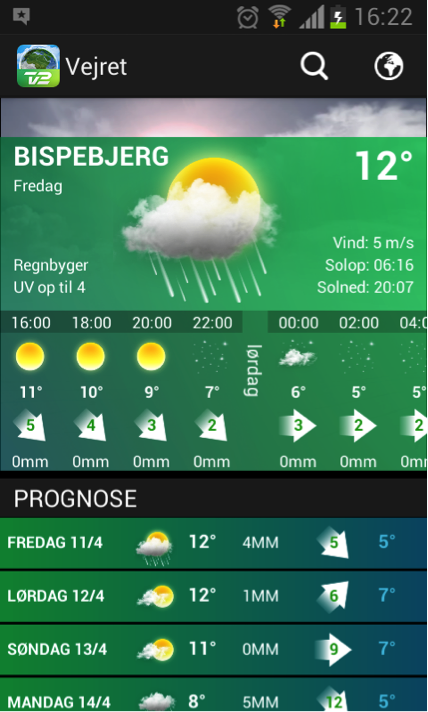
\includegraphics[width=.4\textwidth]{images/Tv21.png}
    \caption{TV2 weather app}
    \label{fig:tv21}
\end{figure}

The app does not however provide radar, heat maps or other more advanced features. 
It has the typical amount of information about the weather for an app, but where the app sets itself apart from the competition, is due to the fact that it is a TV-channel app. 
This means that the app contains video streams of the latest weather forecasts from TV, and other weather related news. 
This can be useful if you want a more detailed forecast with certain highlights about the current and forthcoming weather. 

% subsubsection tv2_vejret_app (end)


\subsubsection*{Yahoo Weather} % (fold)
\label{ssub:yahoo_weather}

Yahoo Weather is an app for iOS and Android which shows the weather in your current location, or if you want, in other locations around the world as well. 
The app contains a lot of the same information that other weather applications do, it is the design of the interface and layout which sets it apart from other apps. 
The application has received the 'Apple Design Award' because of it's aesthetics. 
One of the features of the design, which has gotten a lot of praise, is that the app finds beautiful images of your location on Flickr (an online image database), taking into account the time of the day and current weather condition, of your location and the photos, and uses these as the background of the weather information. 
Aside from this unique approach to visually presenting you surroundings, the interface itself was also very well received by critics. 


In addition to having a very manageable interface, the app actually also contains a great deal of detailed weather information. This data includes:

\begin{itemize}
    \item Temperature
    \item Cloud cover
    \item Precipitation
    \item Probability of downpour (percentage)
    \item Wind Speed
    \item Wind direction
    \item Pressure
    \item Chill factor
    \item Humidity
    \item Visibility
    \item UV-index
    \item Sunrise/sunset
    \item Moon position
    \item Heat map
    \item Wind map
    \item Satellite map
\end{itemize}

Again, as with the TV2 Vejret app, most of the detailed information is only available for the current time on the current day. 
For the 5 and 10 day forecasts there is only information about:

\begin{itemize}
    \item Cloud cover
    \item Day/night temperature peaks
\end{itemize}

Because of the apps very minimalistic design approach the screen is not overloaded with all sorts of data about the weather.
It uses subtle animations  eg. a windmill spinning at a rate according to the current wind speed to illustrate more palpable information about the wind speed. 
Another way the application tries to present information relevant to the user, is by adding customization. 
The user can drag the different 'modules' around to bring the most viewed ones to the top of the screen, limiting the amount of scrolling around to get information you want.

\begin{figure}[!htbp]
    \centering
    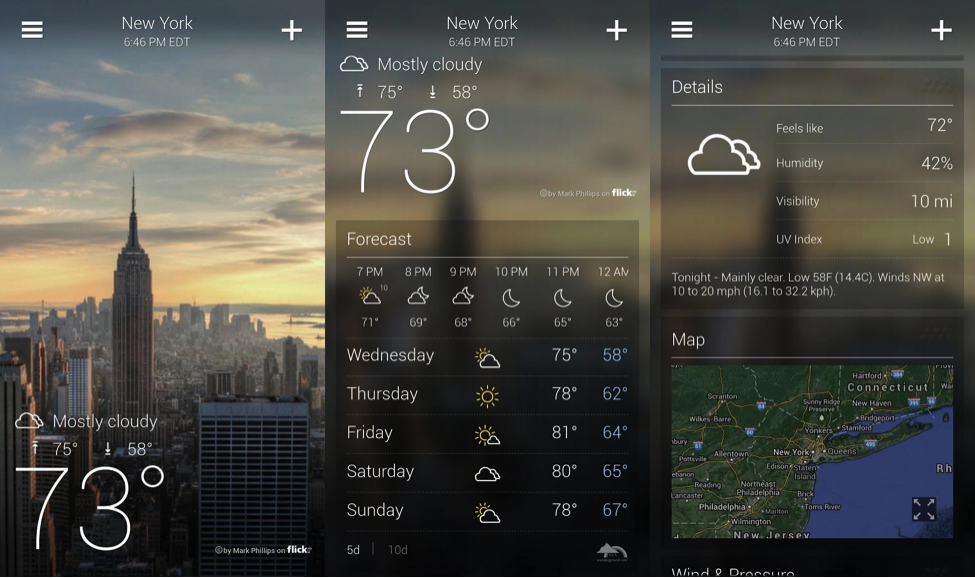
\includegraphics[width=0.95\textwidth]{images/Yahoo1.png}
    \caption{Yahoo weater app}
    \label{fig:yahoo1}
\end{figure}

So all in all, the app does contain a lot of information about the weather, and instead of the developers delimitating the information and deciding which weather data i relevant to the user, they allow the user the option of customizing the app, deciding themselves what information is relevant. 

% subsubsection yahoo_weather (end)


\subsubsection{InstaWeather} % (fold)
\label{ssub:instaweather}

InstaWeather is a weather application that focuses a lot on being a visual application. 
The amount of information about the weather depends on which skin to the application that you want to use. 
The information given can be limited to only being the temperature, a symbol that shows the weather condition and a small forecast. 
Some skins can also be very detailed and give information air pressure, temperature, rain, wind power and direction. 
The app is very customizable so you can change pictures so it feels more personal. 
The main feature in this application is that it borrows the picture sharing ability from Instagram. 
This means that the user can take a picture and send it to a friend with weather information added to the picture.  

\begin{figure}[!htbp]
    \centering
    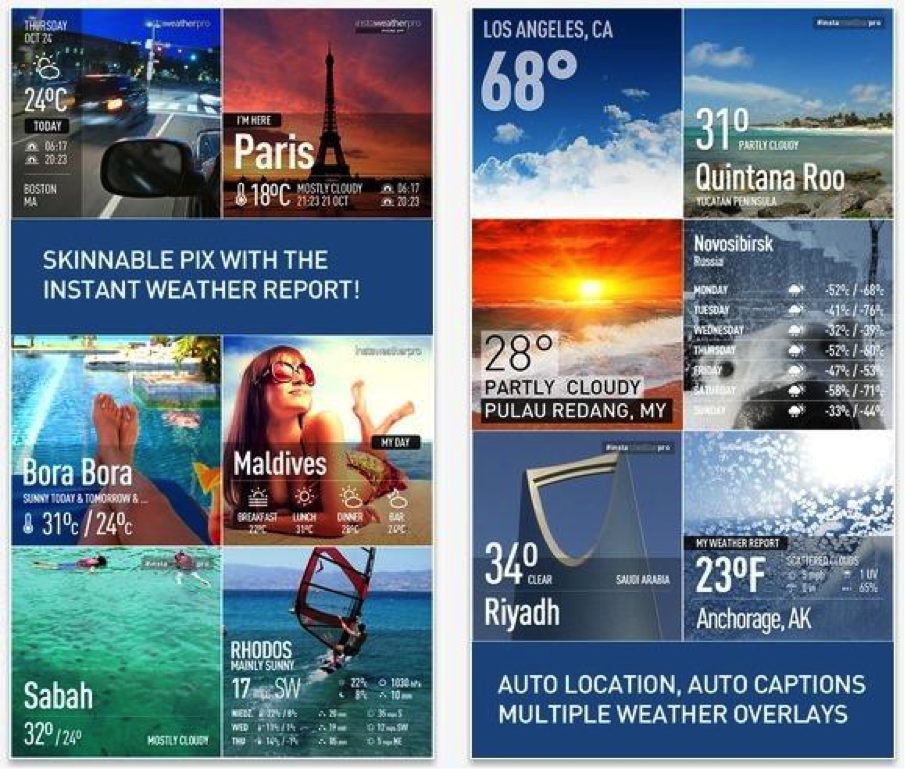
\includegraphics[width=.7\textwidth]{images/Instaweather1.png}
    \caption{InstaWeather}
    \label{fig:instaweather1}
\end{figure}

It is difficult to write about what relevant weather information is in regards to this application, because the user wholly decides for him/her self, what that is. 
It is in some way the most relevant weather information can be to a specific user, if that person puts in the time to customize the application for his or her needs. 
It does not however tell us much about what is in general considered to be chosen as relevant weather data.

% subsubsection instaweather (end)

% subsection weather_data (end)


\subsection{Final Problem Statement} % (fold)
\label{sub:final_problem_statement}

After researching sonification and relevant weather data we find that there are many different ways of using sonification to present different types of data. 
The various weather information from the different sources researched, can be presented in different ways through sonification, but some of the data could prove more challenging to sonify. 
In order to investigate to what extend we can convey these data as non-speech sound, through the use of sonification, the presented information will be compared to the more typical, visual way of presenting these, to figure out if the data can be intuitively understood as sound effects.


\textit{``To what extent is it possible to convey weather information, solely as a nonspeech auditory display, using sonification techniques, and be as intuitively understandable as visually presented weather information, where intuitive is defined as knowing by intuition?''}

% subsection final_problem_statement (end)

% section preanalysis (end)

%!TEX root = ../main.tex

\section{Analysis} % (fold)
\label{sec:analysis}

\subsection{Advantages and Disadvantages of Sonification} % (fold)
\label{sub:advantages_and_disadvantages_of_sonification}

Advantages of sonification are many. 
Not only can we represent data and learn patterns and cycles in said data, but we can also aid the disabled and assist workers in different fields with sound patterns and alarms (Section~\ref{sec:preanalysis}).
However, as with everything there are certain disadvantages of sonification. 
The disadvantages can all be lead from the same disadvantages that sound has. 
Sound can be frustrating or annoying for some users, as people are forced to impose their own taste and ideas subjectively on data. 
Sound is also incredibly hard to describe in certain cases, you cannot mimic sound or make others interpret data without them being able to hear it. 
Listening to sound representing data can require learning or inherent talent, and this learning can take a longer time than looking at visually represented data, although that depends on the type of data. 
The type of data represented also needs to be taken into account for whenever a sound or pattern is chosen. 
\enquote{It is hard to represent a spatial arrangement with sound. You need to use the appropriate display.}
Said Bruce Walker, a professor in the schools of psychology and interactive computing at Georgia Tech, running a group called the sonification lab~\cite*{Feder2012}.

To give a more concrete example of an advantage, sonification was used to study a model of an artificial heart pump, where a modulated sound was indicating pressure on a pusher plate, and a tapping sound indicated a blood cell entering threshold vorticity, and a drum indicated the opening and closing of heart valves. 
It was reported that it seemed easier to determine different things, such as the frequency of blood cells crossing and detecting whether or not the heart valves were opening or closing. 
This is in contrast to the standard method of looking at change in color on a monitor. 
Another example is sonification used to indicate seismic events caused by the fracturing of rock walls during a 3 month dig.
The engineers had a visualization to indicate these fractures, but the events were short and to address this, they added a short sound that varied in volume depending on the magnitude of the event. 
The sounds would draw more attention to periods with more seismic activity, making it easier to detect overlapping events that indicate higher risk. 
Sounds are extremely useful when variables do not appear together in the same image, or require shifting visual attention from monitor to monitor. 
From these two examples, it is clear that when dealing with data that has a variety of events or over longer periods of time, using sound can make the data easier to comprehend.


\subsubsection{Weather data represented using sound} % (fold)
\label{ssub:weather_data_represented_using_sound}

Engineers use visualizations to represent a large amount of data over complex systems, an auditory display can be useful in these cases, where the interpretant needs to keep his eyes focused on the visual data while also receiving data from an audio source. 
The quality and completeness of a fluid flow simulation was analyzed by comparing the sonified audio data generated by a simulated turbine and an actual recording of a turbine~\cite*{Barrass1999}.

Sounds can make it easier to perceive cycles and rhythm, and also abnormalities in a large amount of data. 
Another example of a visualization designed by Simon Kravis at the CSIRO was made to assist the engineers planning a water treatment, works by using a computer model. 
Chemical concentrations in the river’s water are shown by various colored segments, according to the downpour over a one year period. 
They realized that it is difficult to watch the downpour graph and the river visualization at the same time, so they decided to add sonification to represent the downpour so that an engineer may pay less visual attention to the river, while quantities of the downpour are represented by rain-like sound. 
The result of this was that after several repetitions, an engineer could learn the patterns of the rainfall over the year and can anticipate cycles in downpour or dryness. 
The sound representation is meant to bind the different sets of visualizations together and make it easier to remember, and an engineer was able to make relations between chemicals that are never seen at the same time~\cite*{Barrass1998}. 

% subsubsection weather_data_represented_using_sound (end)

% subsection advantages_and_disadvantages_of_sonification (end)


\subsection{Analogic vs Symbolic representation} % (fold)
\label{sub:analogic_vs_symbolic_representation}

There are many different ways to go about designing something that uses sonification. Methods for designing auditory displays have been classified along a spectrum between analogic and symbolic by Kramer~\cite*{Barrass1999}.
\enquote{An analogic representation is one in which there is an immediate and intrinsic correspondence between the sort of structure being represented and the representation medium.}
Meaning, there is one to one mapping between points in the data and points in representation space~\cite*{Barrass1999}. 
Examples for this include a Geiger counter or an auditory thermometer.

Its counterpart, symbolic representation, categorically denotes the thing being represented and relations within the representation do not necessarily reflect intrinsic relationships in what is being represented. 
Examples of a display like this are computer beeps, cellphone alarms and vehicle control notifications.

% subsection analogic_vs_symbolic_representation (end)


\subsection{Semiosis} % (fold)
\label{sub:semiosis}

Semiotics is the study of signs and their creation and interpretation. 
Signs can be anything from images to words, sounds and smells. 
These signs have no inherent meaning other than the one we attribute to them. 
Modern semiotics is based on the work of two major figures, Ferdinand de Saussure and Charles Sanders Peirce, a Swiss linguist and an American scientist respectively~\cite*{Vickers2012}.
In Saussure’s view the sign system is a dyadic relationship between a \enquote{signifier} and a \enquote{signified}.
A signifier is typically a sound pattern, and a signified is the meaning that signifier carries. 
An example of this is the symbol \texttt{/cat/}, which in this case is a signifier for the concept or meaning that we know as a cat. 
The link evoked between the sound pattern and the meaning is the resultant sign. 
Peirce considered this relationship to be insufficient, and he proposed another scheme in which an object referred to is represented by a \enquote{representamen} which then evokes in the mind of the listener the meaning of the sign which he refers to as the \enquote{interpretant}. 
The two theories loosely refer to one another and can be shown as such~\cite*{Vickers2012}(Figure~\ref{fig:semiosis1}):

\begin{figure}[!htbp]
    \centering
    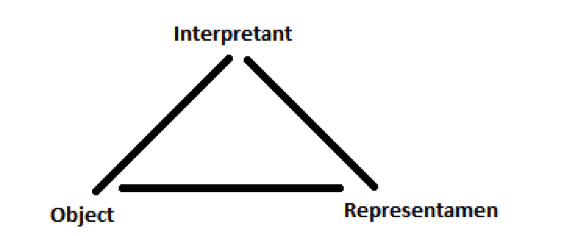
\includegraphics[width=.5\textwidth]{images/Semiosis1.png}
    \caption{XX}
    \label{fig:semiosis1}
\end{figure}

% subsection semiosis (end)


\subsection{Sonification usage} % (fold)
\label{sub:sonification_usage}

Sonification can be split up in 4 different kinds of function types, when going by theory created by Bruce N. Walker and Michael A. Ness~\cite*{walker2011}. 
The 4 different types are as follows: 

\begin{enumerate}
    \item Alarms, alerts, and warnings
    \item Status, process, and monitoring messages
    \item Data exploration
    \item Art and entertainment
\end{enumerate}


\subsubsection*{Alerting functions} % (fold)
\label{ssub:alerting_functions}

Alerting functions refers to sound indicating that a certain event is occurring or has occurred, but it usually won’t convey descriptive data on the alerted subject. 
For example, a microwave oven makes a beep when the timer has expired, but it will not tell you if the containing substance is done or overcooked. 
Another example is the usage of calendar notifications on phones or tablets. 
These notifications will only notify you that something is going to happen by ringing or beeping. 
To further understand what the occurring sound means, a visual clue or a memory of the upcoming event is required.

The last example in this category is a fire alarm. 
A fire alarm will ring loudly to alert you that you need to move immediately, in most cases out of the building, but it does not contain any information about the location of the fire, nor does it tell you how severe the fire is.

% subsubsection alerting_functions (end)


\subsubsection*{Status and progress functions} % (fold)
\label{ssub:status_and_progress_functions}

Status and progress function has a purpose similar to that of alerting functions, but to understand the data correctly, a visual display or another form of continuous data is required to fully understand the situation at hand. 
It requires the interpretant to pay attention to small changes in the auditory feedback. 
This relates to the example given (Section~\ref{sec:preanalysis}) that we have previously discussed, where surgeons focus their eyes on the patient while listening to the heart monitors.

When designing a weather application, this could be the function to use if your goal was to have mostly visual data, only supplied by auditory data. 
However, it is important to note that when using this type of sonification, the auditory display itself is only a sub part of the data. 

% subsubsection status_and_progress_functions (end)


\subsubsection*{Data exploration functions} % (fold)
\label{ssub:data_exploration_functions}

When talking of sonification, this is the function usually referred to. 
Data exploration is meant to encode and convey information about entire sets of data, or relevant aspects of said data.
Sonification designed for data exploration is different from status or process indicators, seeing as they use sound to offer a more \enquote{holistic portrait} of the data, as opposed to condensing information to capture a momentary state~\cite*{walker2011}.

% subsubsection data_exploration_functions (end)


\subsubsection*{Art and Entertainment} % (fold)
\label{ssub:art_and_entertainment}

Since the sound producing capabilities of computers have evolved exponentially over the past years, so have the music producing of computers too. 
Sound data like sonification have been adapted more and more in to the world of music, and more artist uses data mapping included in their song or tracks. 
Since music does not really convey any form of information, it can still be included in the sonification functions, since it still conveys the expression/data of art and entertainment.

The above covers the different sonification functions, and in which cases they can be useful to alert or notify interpretants.

% subsubsection art_and_entertainment (end)


As you read above sonification have a lot of functioning abilities, as to how you can use audification without speech to notify a user what happens around them without using their eyes or hands, but sonification can also be categorized in their techniques and how you approach them. 
So far we have only explained what sonification can be used for, but not how the techniques are in practice, does it require interaction from a user or not?. 
Those approaches can be categorized in 3 categories which are (1) event based, (2) Model Based (3) Continuous.


\subsubsection*{Event-based sonification} % (fold)
\label{ssub:event_based_sonification}

The Event based approach is where the data of the sonification display is employed by the parameter mapping. 
Parameter mapping are changes in data dimension with changes in an acoustic dimension to produce a sonification. 
Parameter sees changes in data and then try to convey that data with as much as a feasible display through sounds, to show what that data means, a lot like what we want to do with data of the weather. 
The event based approaches have more or less through time, had a passive interaction possibility with brief notification like alarms and notification, but event based sonification that employ parameter mapping have the possibility to adapt to both passive and active interaction.

The sonification Handbook~\cite[363]{Hermann2011} shows several examples to sound that tells the user e.g. that their target destination is reached.
The data will read the remaining length of the journey and then intensify the sonification/sound depending on how close you are to your target.

% subsubsection event_based_sonification (end)


\subsubsection*{Model-based sonification} % (fold)
\label{ssub:analysis_model_based_sonification}

Model based differs from event based a lot, since here you need a virtual model that relies heavily on the interaction between the user and the virtual object. 
The virtual object then reads the users interaction, and converts that interaction into sonification. 

The Sonification Handbook video number 16.3~\cite*[410]{Hermann2011} shows a perfect example of model based sonification. 
You see a user with a triangular object moving around, the software then detects his movement and convert his actions in to sounds depending on how the object is moved. 
Another example of this can be a metal detector, which some people uses on the beach to scavenge forgotten objects on the beach. 
The metal detector will notify/alarm you if your metal detector senses any metal beneath its reader. 

% subsubsection analysis_model_based_sonification (end)


\subsubsection*{Continuous sonification} % (fold)
\label{ssub:continuous_sonification}

Continuous sonification is possible when data are timed series and sampled at a rate that a quasi-analog signal can be directly translated in to sound (quasi-analog signal in telecommunication is a digital signal that has been converted to a suitable form for transmission through analog channel). 
To explain it more simply is when sound waves are directly translated in to sound. 
That means the sonification happens when the software translate the data from a sound wave in to sound e.g. a Richter scale converts seismic data in to wave forms, that can then show the seismic event with a 90\% accuracy.

% subsubsection continuous_sonification (end)


The group will generally focus on the first approach of sonification (event based), since the task for our idea is to notify the user, what he/she can expect the weather condition to be for the day or notify the user that its going to rain in X minutes, and by using parameter mapping we can also change the sound output dependent on the data of the weather condition, and ideally it will make a sound that the user can understand how warm or how cold it is outside, by just hearing a sound.

% subsection sonification_usage (end)


We now know that sonification can notify you in many different ways, that some forms require a passive listener and some requires and active listener, maybe both. 
The approaches for sonification is also different depending on the task or the message that you which you convey, and that sonification can also have interaction methods that require the user to physically interact with an object to generate sonification to work. 
The group now needs to work out what kind of sonification function and techniques that need to be implemented in to our project and work from there.

% section analysis (end)

%!TEX root = ../main.tex

\section{List of Requirements} % (fold)
\label{sec:list_of_requirements}

The content of the list of requirements is to be seen as parameters for the product design. 
The arguments have been refined in the analysis-chapter, and have ultimately led to these requirements, that will help construction of the final product. 
Hence it is to be considered a blueprint from which numerous variations of designs can be crafted.

General requirements:
\begin{itemize}
    \item The prototype must contain sounds that range in different levels within the same weather category.
    \item The visuals provided in testing must be based on results from either pre-testing or SOTA analysis.
\end{itemize}

Program functionalities:
\begin{itemize}
    \item Able to import sound file
    \item Able to play sound file
    \item Able to pause sound file
    \item Able to change the tempo of the sound
    \item Able to add filters to the sounds
\end{itemize}

What we hope to achieve from the test:

\begin{itemize}
    \item People are able to understand the sounds
    \item People are able to understand the pictures of the different weather categories
\end{itemize}
% section list_of_requirements (end)
\include{./chapters/methods}
%!TEX root = ../main.tex

\section{Design} % (fold)
\label{sec:design}

In this chapter we will look at the design of the prototype, which will be used in our test with the purpose of answering the final problem statement. 
The design will be based on the list of requirements (see chapter \ref{sec:list_of_requirements} for the list of requirements). 
We are also going to take a look at the delimitation of our weather categories (e.g. temperature, wind speed, precipitation...). 
Based on the requirements and delimitation, pre-tests will be designed and carried out. 
These tests will then lead into a design blueprint of our prototype.

From the list of requirements it should be possible to plan how the prototype is going to fulfil all of the specific requirements. 
Additionally, the weather categories have to be delimited into a realistic amount of weather conditions which suits our timetable. 
After the delimitation, the visual and auditory elements will be chosen from the results of pre-testing, whereof the pre testing determines the sounds and visual elements which will later be used in the actual implementation. 
When the sounds and pictures are in place, it is time to create the blueprint of what the pictures should look like and how the sounds are going to be made. 
Figure~\ref{fig:design1} describes the process of the actual design of the prototype.

\begin{figure}[!htbp]
    \centering
    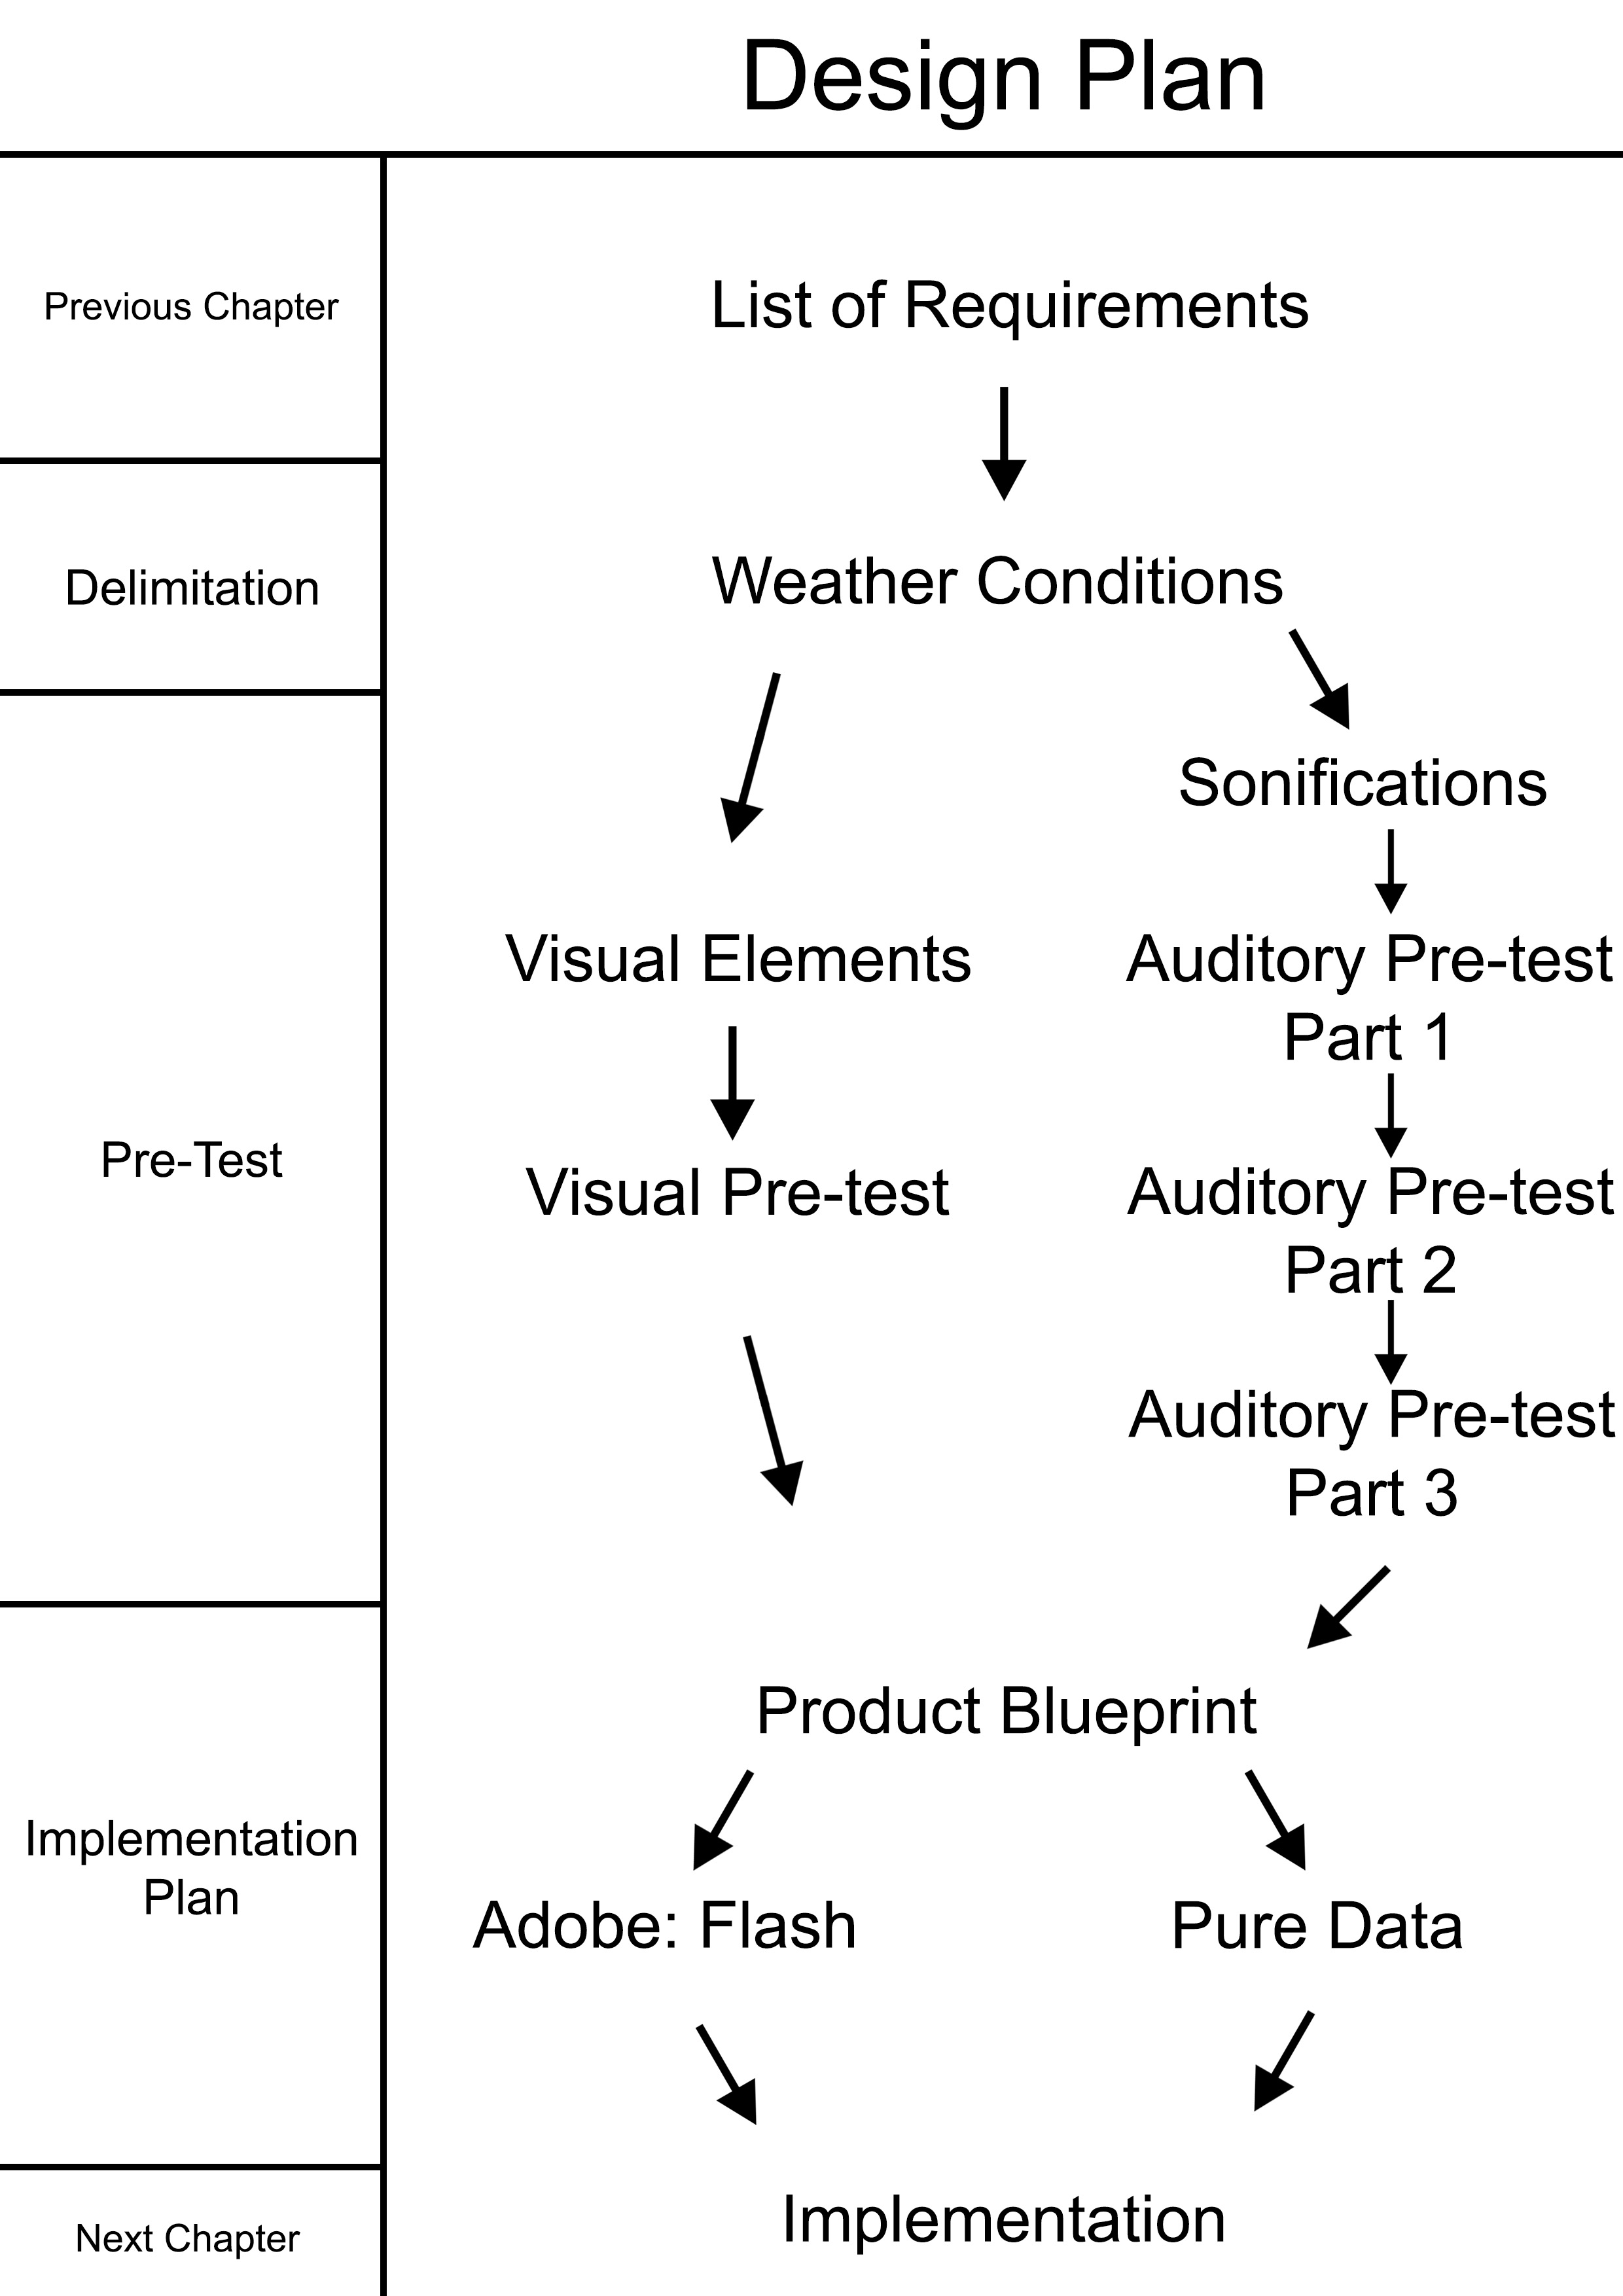
\includegraphics[width=.5\textwidth]{images/Design1.jpg}
    \caption{Plan for design process}
    \label{fig:design1}
\end{figure}


\subsection{A design to meet all the requirements} % (fold)
\label{sub:a_design_to_meet_all_the_requirements}

To get an overview of how the requirements are going to be fulfilled, the requirements have been split up into two categories. Requirements for testing and requirements for the prototype itself.

\subsubsection{Testing} % (fold)
\label{ssub:testing}

General requirements:

\begin{itemize}
    \item The prototype must contain sounds that range in different sound-parameters within the same weather category, such as varying amounts of rain.
    \item The visuals provided in testing must be based on results from either pre-testing and/or SOTA pre-analysis
    \item The sounds must have a meaning attached to them (i.e. semiosis)
    \item Symbolic representation is used to convey our message about the weather
    \item Will use the type “data exploration” of sonification to translate weather data into sound
\end{itemize}

We have decided to have a pre-test to decide on the images to be used in the prototype. 
This test involves test subjects to draw a given weather category (e.g. a drawing of certain amount of wind speed etc.). 
To determine the sounds for the prototype it was decided to make a three-step test. 

First step is to ask test participants what sounds could be used to symbolise the different weather conditions.
The second step was to make a another interview where people had to recognize the sounds that we had chosen, based upon the first pre-test. 
The last pre-test was to establish what value the test subjects associated with the specific weather conditions.

The first two pre-tests define the sounds/sonifications for the weather conditions. 
The last pre-test describes if the sonifications formulate the desired values of each weather condition.

% subsubsection testing (end)


\subsubsection{Prototype} % (fold)
\label{ssub:prototype}

Program functionalities must be able to:
\begin{itemize}
    \item Import sound file
    \item Play sound file
    \item Pause sound file
    \item Change the tempo of the sound
    \item Add filters to the sounds
\end{itemize}

We have decided to use Pure data\footnote{\url{http://puredata.info/}} since we already have some knowledge in this program and know it can fulfil our requirements. 

% subsubsection prototype (end)

% subsection a_design_to_meet_all_the_requirements (end)


\subsection{Weather Conditions} % (fold)
\label{sub:weather_conditions}

There are a lot of different kinds of weather data. 
Since it is not possible to cover every single category of weather data within the projects time limit we decided to make a delimitation of the weather data to what we deemed most relevant. This decision is not based upon prior research.

Based on the research from the weather applications (See Pre-Analysis section~\ref{sub:weather_data}) the following raw weather data list was created.

\subsubsection*{Raw list of weather data} % (fold)
\label{ssub:raw_list_of_weather_data}

\begin{itemize}
     \item \textbf{Temperature/Dewpoint} - Current air temperature 2 meters above terrain.
     \begin{itemize}
         \item Day temperature
         \item Night temperature
         \item Average temperature
     \end{itemize}
     \item \textbf{Wind speed} - Average wind speed over 10 minutes, 10 meters above terrain.
     \item \textbf{Wind direction} - Average wind direction in degrees.
     \item \textbf{Air pressure} - Pressure at sea level measured i hPa (Hectopascal).
     \item \textbf{Humidity} - Current relative humidity measured 2 meters above terrain, measured in percent.
     \item \textbf{Precipitation} - Rain/sleet/snow/hail over the past ten minutes measured in mm.
     \item \textbf{Sun hours} - Hours with sun in a day.
     \item \textbf{Pollen Forecast} - The potency of the pollen. 
     \item \textbf{Sunrise / sunset} - Time of day where the sun rises and sets.
     \item \textbf{Cloud cover}
     \item \textbf{Wind chill} - The winds effect on air temperature.
     \item \textbf{Visibility} - How far can you see with clear line of sight.
     \item \textbf{UV-index} - Intensity of UV radiation.
     \item \textbf{Fronts} 
     \item \textbf{Source Regions} - Where the air is coming from.
     \item \textbf{Drought} - Risk of drought. Presented as a scale.
     \item \textbf{Downpour} - Rain in mm.
 \end{itemize}

After going through the data on the raw list we found that many of the weather categories did not fit the project. 
Therefore, we decided to only use relevant weather data that people normally would use in an everyday situation, whereof relevance is determined by us.
This delimitation is based on our research on which types of weather data there is available in the weather applications (See Pre-Analysis section~\ref{sub:weather_data}).

% subsubsection raw_list_of_weather_data (end)


\subsubsection*{List of relevant data} % (fold)
\label{ssub:list_of_relevant_data}

\begin{itemize}
     \item \textbf{Temperature/Dewpoint} - Current air temperature 2 meters above terrain.
     \begin{itemize}
         \item Day temperature
         \item Night temperature
         \item Average temperature
     \end{itemize}
     \item \textbf{Wind speed} - Average wind speed over 10 minutes, 10 meters above terrain.
     \item \textbf{Wind direction} - Average wind direction in degrees.
     \item \textbf{Humidity} - Current relative humidity measured 2 meters above terrain, measured in percent.
     \item \textbf{Precipitation} - Rain/sleet/snow/hail over the past ten minutes measured in mm.
     \item \textbf{Sun hours} - Hours with sun in a day.
     \item \textbf{Pollen Forecast} - The potency of the pollen.
     \item \textbf{Wind chill} - The winds effect on air temperature.
     \item \textbf{Visibility} - How far can you see with clear line of sight.
     \item \textbf{UV-index} - Intensity of UV radiation.
     \item \textbf{Downpour} - Rain in mm.
 \end{itemize}

Going through the weather data, we decided to make another delimitation. 
The list was further delimited based on our thoughts of what an average person would need to know in an everyday scenario, so the list of data does not necessarily represent the weather categories required to create a functional weather application with appropriate weather categories. 

% subsubsection list_of_relevant_data (end)


\subsubsection*{List of delimited weather data} % (fold)
\label{ssub:list_of_delimited_weather_data}

\begin{itemize}
     \item \textbf{Temperature/Dewpoint} - Current air temperature 2 meters above terrain.
     \begin{itemize}
         \item Day temperature
     \end{itemize}
     \item \textbf{Wind speed} - Average wind speed over 10 minutes, 10 meters above terrain.
     \item \textbf{Precipitation} - Rain/sleet/snow/hail over the past ten minutes measured in mm.
     \item \textbf{Pollen Forecast} - The potency of the pollen.
     \item \textbf{Visibility} - How far can you see with clear line of sight.
     \item \textbf{Cloud Cover.}
     \item \textbf{UV-index} - Intensity of UV radiation.
     \item \textbf{Downpour} - Rain in mm.
 \end{itemize}

% subsubsection list_of_delimited_weather_data (end)


\subsubsection{Categories} % (fold)
\label{ssub:categories}


We did not use Continuous Sonification as specified in the analysis. (See analysis section~\ref{par:continuous_sonification}), because it is hard for people to interpret numbers, for example: \enquote{Could you make a sound based on a temperature of 12 degrees?}. 
Since it is not possible for us to go through every degree of e.g. temperature, the numbers were converted into three categories: Low, Medium and High. 
We also decided that the weather data "Pollen" and "Visibility", should act like a warning indicator. 
This means that the sound should only be played above or below a specific value.
This decision was made since there is no reason to warn users about weather conditions that might affect the user when there is none. 
In this case "Pollen" will be played when there is a high amount of pollen, and "Visibility" will be played when there is low visibility.

When the values had been decided , the values had to be assigned. We are getting our Low, Mid and High value from DMI\footnote{\url{http://www.dmi.dk/vejr/til-lands/byvejr/by/vis/DK/1000/K\%C3\%B8benhavn,\%20Danmark}}. The values are estimates of low, medium and high based on the data from DMI.

\begin{table}[!h]
\centering
\begin{tabular}{l | l | l | l}
Category & Low & Medium & High \\
\hline \hline
Temperature & 0'C & 15'C & 30'C \\
Wind Speed & 5 m/s & 17 m/s & 32 m/s \\
Pollen Forecast & 0 - 30 & & 30 - 100 \\
Visibility & 10 m & & 10 km \\
Downpour & 0 mm & 3 mm & 10 km \\
UV-index & 3 & 3 - 6 & 7 - 8 
\end{tabular}
\caption{Category values}
\label{tab:category_values}
\end{table}
% subsubsection categories (end)

% subsection weather_conditions (end)

\subsection{Visual pre-test} % (fold)
\label{sub:visual_pre_test}

A pre-test was done to identify the common visual associations often used with the weather forecasts, these associations will form a basis for the visual implementations. 
The visual implementation will contain images of certain weather conditions that people should find intuitive.

The test took the form of a simple interview where the subject was asked to draw certain weather conditions.

Because the test has no target group other than people who have at some point checked a weather forecast, the test will be conducted using accidental sampling.
accidental sampling selects every subject in the test from a greater group of subjects (the target group) completely at random. 
Every subject has an equal chance to get picked to do the survey.

The selected subjects would be given a piece of paper with three empty frames. 
The subject was then asked to draw the first thing that came to mind when told about a weather condition. 
A sample question could be: \enquote{draw the first thing that comes to mind when i tell you that it is 30*C outside}. 
The subject would then draw their association. 
The subject would then be asked to make another drawing of the same weather condition but with a different value. 
i.e. if the subject had first been asked to draw a hot day, they would then be asked to draw a cold day and then an average day.

5 people for each weather condition was asked to participate, 35 in total. 
The complete drawing sheet and answers to the survey can be found in appendix~\ref{sec:visual_pre_test_raw_results}.

\begin{table}[!htbp]
    \centering
    \begin{tabular}{l | l | l | l}
    Condition & Value & Possible solution & Alternate solution \\
    \hline \hline
    Temperature & Low & Snowflake, snow &  \\
    & Medium & Average clothing \\
    & High & Sun and beach & Thermometer \\
    \hline
    Downpour & Low & Sunny & Clouds, no rain \\
    & Medium & Clouds with rain & \\
    & high & Clouds with much rain & \\
    \hline
    Wind speed & Low & Tree/Flag, no movement & \\
    & Medium & Tree/flag, some movement & \\
    & High & Tree/man, much movement & \\
    \hline
    Pollen & Low & Man, happy/smiling & \\
    & Medium & Man, Sneezing & \\
    & High & Man w. runny nose, red eyes, itching & \\
    \hline
    Visibility & Low & Window, gray outside & \\
    & Medium & Gray colors & cloudy \\
    & High & Clear day, sun & \\
    \hline
    Cloud cover & Low & Clear day, sun & \\
    & Medium & Few Clouds & \\
    & High & Overcast & \\
    \hline
    UV-index & Low & Cloudy day & \\
    & Medium & Clouds, sun & \\
    & High & Sun, no clouds & \\
    \end{tabular}
    \caption{Possible visual implementations}
    \label{tab:visual_pre_test}
\end{table}

Table~\ref{tab:visual_pre_test} shows the possible solutions for the visual implementation based on the acquired results.
The drawings were analyzed for common traits within the same condition and value, i.e. if two or more drawings of the same condition and value would contain a person, this would be interpreted as a possible common association and be included as possible solution.

% subsection visual_pre_test (end)

\FloatBarrier
\subsection{Sound pre-test} % (fold)
\label{sub:sound_pre_test}
The idea of the pre-test is to determine what sounds to choose when looking for the optimal choice of sounds to use the designated sonifications of each weather condition. 
We will go through a three step audio pre-test that will provide us with the information we need. 
The first step is meant to give us insight about what sound to use. 
The second step is to test these previously mentioned sounds to see if people recognize what it is meant to represent. 
The third step is to play the sounds to the test subjects and then ask what weather data these sounds represent, in a setting where we have already specified the weather category, to figure out if the specified sound also formulates the designated value of the weather condition.

\subsubsection{Audio Pre-Test - Part One} % (fold)
\label{ssub:audio_pre_test_part_one}
This first part of the pre-test was meant to give an idea of what sounds to use according to the feedback given from interviews. 
We then provide our own thoughts in addition to determine what the sounds should be.

\paragraph{Purpose} % (fold)
\label{par:purpose} 
\hspace{0pt} \\
Determine what sounds to use in each of the weather condition categories as specified in the list of delimited weather data. See \ref{ssub:list_of_delimited_weather_data}

% paragraph purpose (end)

\paragraph{Description} % (fold)
\label{par:description}
\hspace{0pt} \\
Part one was performed by interviewing people randomly selected around the AAU campus. 
This part of the pre-test contains questions about how the testers would describe the different weather categories with a sound or a scenario, both for high and low values of the specific weather conditions. 
This information is then used to acquire/develop the sounds for the pre test, where the actual sounds will be tested to see if they represent the answers acquired from this test.

\begin{tabular}{l l}
Amount of participants: & 12 test participants \\
Test subject sampling: & Convenience sampling: Aalborg University students. \\
Estimated length of test: & Around 10 min per test subject. \\
Test location: & Area on and around Aalborg university. \\
Date and time: & When appropriate.
\end{tabular}

% paragraph description (end)

\paragraph{Results} % (fold)
\label{par:results}
\hspace{0pt} \\
See appendix~\ref{sub:pre_test_1_results} for results.

These results have been placed together for each category, where you can see answers for both high and low values. 

% paragraph results (end)

\paragraph{Evaluation} % (fold)
\label{par:evaluation}
\hspace{0pt} \\
When analyzing the data that has been gathered, it was seen that most of the categories have the same answers. 
Our sounds were based on a mix of how the majority wanted the sounds to be like and what we believed could be a recognizable sound. 
The following is an overview of our thought process. 

\subparagraph{Temperature} % (fold)
\label{subp:temperature}
\emph{High:} We noticed that a high pitched sound was a frequent answer among the participants. We went with this in mind when choosing the soun. 
The sound that we ended up choosing, was inspired by one of the participants that answered \enquote{a boiling kettle}. \newline
\emph{Low:} The majority answered \enquote{breaking ice} and \enquote{snow}, but since we are using that for Precipitation - Snow it is not an option. 
We instead went with the \enquote{teeth grinding} sound.
% subparagraph temperature (end)

\subparagraph{Wind Speed} % (fold)
\label{subp:wind_speed}
\emph{High:} A \enquote{high wind gust} seemed to be the most common answer, so that is what we went with.
\emph{Low:} A \enquote{low wind gust} seemed to be the most common answer, so that is what we went with.
% subparagraph wind_speed (end)

\subparagraph{Precipitation} % (fold)
\label{subp:precipitation}
\emph{Rain:} All the answers to this were \enquote{rain}, so we went with rain as our sound.
\emph{Snow:} Most of the answers to this were \enquote{snow}, but since snow does not have a sound then we went with footsteps in the snow.
\emph{Hail:} All the answers to this were \enquote{hail}, so we went with hail as our sound.
% subparagraph precipitation (end)

\subparagraph{Pollen Forecast} % (fold)
\label{subp:pollen_forecast}
\emph{High:} \enquote{A sneeze} was the most common answer, so that is what we chose as our sound.
\emph{Low:} Because we are going with pollen as a warning indicator this question was only stated to satisfy our curiosity. 
The test participants did not give any real responses to this question. 
% subparagraph pollen_forecast (end)

\subparagraph{Visibility} % (fold)
\label{subp:visibility}
\emph{Low:} Most of the people we asked described a foggy scenario as seen in movies. 
Since this is the scenario most people think of, we chose a \enquote{fog horn} sound to remind them of this scenario in the hopes that they would associate it with a foggy day.
% subparagraph visibility (end)

% paragraph evaluation (end)

% subsubsection audio_pre_test_part_one (end)


\subsubsection{Audio Pre-Test - Part Two} % (fold)
\label{ssub:audio_pre_test_part_two}

\paragraph{Purpose} % (fold)
\label{par:pre_test_2_purpose}
\hspace{0pt} \\
The second part of the pre-test is based upon the results given from pre test 1 (See section~\ref{ssub:audio_pre_test_part_one}). 
The results has been evaluated, and sounds that could be used as a sonification of the specific weather conditions has been found/developed. 
The following test is conducted as we want to ensure that the chosen sounds actually represent the results from the previous test and can be used in the designated prototype. 
The test will elaborate upon the sounds and will make it possible to evaluate whether the sounds are understood or not, and what the test subjects think that the sounds intuitively implies.
% paragraph purpose (end)

\paragraph{Description} % (fold)
\label{par:pre_test_2_description}
\hspace{0pt} \\
The procedure of the test was conducted in the following manner. 
A single test subject was asked to listen to the acquired/constructed sounds, and was then asked to write down what he/she relates to the sound e.g. what the subject thought of the sound actually implies. 
The test subject was given no prior information to the test, and was unaware of everything but the test procedure.
This ensured that the test subject was given no information that could be used to assume anything based upon the sounds and somewhat bias the results, as we were looking for the intuitive understanding of the presented sounds.

\begin{tabular}{l l}
Amount of participants: & 10 test participants \\
Test subject sampling: & Convenience sampling \\
Estimated length of test: & 10 min per test subject. \\
Test location: & Area on and around Aalborg university. \\
Date and time: & When appropriate.
\end{tabular}

% paragraph description (end)

\paragraph{Results} % (fold)
\label{par:pre_test_2_results}
\hspace{0pt} \\
See appendix~\ref{sub:pre_test_2_results} for the acquired test results.

\enquote{List of sounds} represents the sounds that were played to each individual test subject in that specific order.
\enquote{Test x} represents answers written down from each test participant in each column, where the data represents the denoted answer from the test participant.
The right sided column to each test section represents the interpretation of results.

The result interpretations are divided into three categories: \newline
\textbf{Correct} - Represents a correct answer. \newline
\textbf{Correct()} - Represents an answer that is associated with the correct answer, as decided by us, and is therefore marked as correct. 
The associations are deemed correct by us and does not represent a scientific decision. \newline
\textbf{Incorrect} - Represents an incorrect answer. 
Either the sound was not guessed, indicated by \enquote{-}, in the test results, or the responses was not in any way associated with the sound, as deemed by us.

% paragraph results (end)
\pagebreak[3]
\paragraph{Evaluation} % (fold)
\label{par:pre_test_2_evaluation}
\hspace{0pt} \\
Table \ref{tab:pre_test_2_evaluation} illustrates the amount of correct answers in percentages.

\begin{table}[!hb]
\centering
\begin{tabular}{l l r c}
   & Sound &  Answered correctly & \\
\hline
1. & Hail - Downfall hail & 70\% & 7/10 \\
2. & Rain - Downfall rain & 100\% & 10/10 \\
3. & Snow - Downfall snow & 10\% & 1/10 \\
4. & Birds - Downfall nothing & 60\% & 6/10 \\
5. & Horn - Fog & 90\% & 9/10 \\
6. & Sneeze - Pollen & 90\% & 9/10 \\
7. & Kettle - High temperature & 90\% & 9/10 \\
8. & Clattering Teeth - Low temperature & 0\% & 0/10 \\
9. & Small breeze - Medium temperature & 70\% & 7/10 \\
10. & Wind - Wind speed & 100\% & 10/10
\end{tabular}
\caption{Pre-test 2 evaluation}
\label{tab:pre_test_2_evaluation}
\end{table}

\begin{enumerate}
    \item \textbf{Hail} - The majority of test subjects answered \enquote{hail}, which was the desired implication of the sound. 
    We suspect that when the test subjects are aware of the subject, being weather - and thereafter will have to guess what the sound implies - the sound will suffice.
    \item \textbf{Rain} - All test subjects answered correctly, therefore the sound is deemed to require no alterations or changes.
    \item \textbf{Snow} - A low amount of test participants, around 10\%, was able to associate the sound with snow as intended. We therefore chose to replace the sound.
    \item \textbf{Birds} - A majority of 60\% answered correctly. This indicates that while most answers correct, adjustments might ensure that a larger percentage of test subjects will answer correct. Plausible alterations will be decided by us.
    \item \textbf{Horn} - A Majority of 90\% answered correctly. Therefore no alterations will be made.
    \item \textbf{Sneeze} - A Majority of 90\% answered correctly. Therefore no alterations will be made.
    \item \textbf{Kettle} - A Majority of 90\% answered correctly. Therefore no alterations will be made.
    \item \textbf{Teeth} - No test participants were able to answer correctly. Therefore we will replace the sound.
    \item \textbf{Small breeze} - The majority of 70\% was able to answer correctly. Adjustments will be made, and might ensure that a larger percentage of the subjects will be able to answer correct. Plausible alterations will be decided by us.
    \item \textbf{Wind} - All test subjects answered correctly, therefore the sound is deemed to require no alterations or changes.
\end{enumerate}

% paragraph evaluation (end)

% subsubsection audio_pre_test_part_two (end)

\subsubsection{Audio Pre-Test - Part Three} % (fold)
\label{ssub:audio_pre_test_part_three}
Since the previous part of the pre-test we replaced the LowTemp sound (Teeth) with a new sound that has been tested around the campus and is being deemed ready for use. 
A small delimitation has also been made to downpour. 
It now only covers rain since we encountered a problem that we didn’t think about at the early stages. 
The problem was that we designed downpour to be changed by play speed of the sound, and the only sound capable of being modified in this manner is rain.

Now that every sound has been deemed ready for use, we are able to proceed into the third step of the pre-test. 
In this step we are going to play the sound and give information about what weather category it is. 
We then want our testers to answer what weather data type they believe the sound represents.  

\paragraph{Purpose} % (fold)
\label{par:pre_test_3_purpose}
\hspace{0pt} \\
The purpose of this part of the pre-test is to make sure that our sounds are recognisable with a weather data type when combined with a weather category.
% paragraph purpose (end)

\paragraph{Description} % (fold)
\label{par:pre_test_3_description}
\hspace{0pt} \\
\begin{tabular}{l l}
Amount of participants: & 10 test participants \\
Test subject sampling: & Convenience sampling \\
Estimated length of test: & 15 min per test subject. \\
Test location: & Ballerup, Albertslund, and Aalborg university. \\
Date and time: & When appropriate.
\end{tabular}
% paragraph description (end)

\paragraph{Results} % (fold)
\label{par:pre_test_3_results}
\hspace{0pt} \\
See appendix \ref{sub:pre_test_3_results} for results.

On this list it can be seen what each test person answered to the sounds.
% paragraph results (end)

\paragraph{Evaluation} % (fold)
\label{par:pre_test_3_evaluation}
\hspace{0pt} \\
Most of our sounds were recognisable and provided the people testing with the intended information. \newline
There were a few sounds (listed below) that gave us some negative data.

\subparagraph{TempMed:} % (fold)
\label{subp:tempmed_}
People gave many different answers for this sound. 
This is a problem and this sound has to be replaced and tested once more.
% subparagraph tempmed_ (end)

\subparagraph{Pollen:} % (fold)
\label{subp:pollen_}
Most of the people got the correct weather category but some also answered \enquote{cold}. 
Since it is a sneeze this is something that we should have expected. 
We will try to modify the to make sure that test participants make a clearer association to pollen. 
% subparagraph pollen_ (end)

\subparagraph{Fog:} % (fold)
\label{subp:fog_}
All the people that answered the question got the answer correct. 
However, we also had some people who were unable to answer the question. 
We conclude that they might know what the sound is, but they do not manage to connect it into that foggy scenario that we imagined people would in the first part of the pre-test.
% subparagraph fog_ (end)

% paragraph evaluation (end)

After making the proper adjustments to the sounds, we feel that we are at this point ready to implement them, and use them for further testing.

% subsubsection audio_pre_test_part_three (end)

% subsection sound_pre_test (end)

\FloatBarrier
\subsection{Product Blueprint} % (fold)
\label{sub:product_blueprint}

Now that the visual and auditory elements have been determined, it is time for us to plan how to make use of the acquired data.

\subsubsection{Visual Elements} % (fold)
\label{ssub:visual_elements}

The visual design is based on the table from the visual pre-test (Table~\ref{tab:visual_pre_test}). We use the information from our user pre-test, where to test subjects had to draw how they imagined a certain weather condition to be illustrated, to come up with similar illustrations for weather conditions in the prototype.

% subsubsection visual_elements (end)


\subsubsection{Audio elements} % (fold)
\label{ssub:audio_elements}

When the different sounds for weather categories were in place, the next step was to figure out how to make these sounds fit into our value categories. 
Most of the sounds can be placed and played under the fitting values, but rain (Downpour) and wind speed had to be changed in order to let people know if it had a low, medium or high value.
In order to change these sounds we decided to use Pure Data.
With Pure Data it was possible to change the speed of the sound and add filters so the sounds that were able to fit into our value categories.

Here are the Pure Data objects we will use for the implementation:

\paragraph{Band Pass Filter} % (fold)
\label{par:band_pass_filter}

Band Pass Filter also called [bp~] in Pure Data, is a filter that only allows some range of frequencies between the highest and lowest. 
It has three inputs. 
The first one is the input from the audio. 
The second input is for the center frequency that will be allowed to pass. 
The third input is the resonance, which determines how wide the ranges of frequencies that are allowed to pass through the filter are. 
The function is that the center frequency will be unchanged, but the frequencies, higher or lower, will be reduced or removed from the sound.

% paragraph band_pass_filter (end)


\paragraph{Sample} % (fold)
\label{par:sample}

A sample refers to a value or multiple values that is set to a point in time.

% paragraph sample (end)


\paragraph{Metro} % (fold)
\label{par:metro}

An object that keeps calling after a specific amount of time (in milliseconds).

% paragraph metro (end)
    

\paragraph{Phasor} % (fold)
\label{par:phasor}

A phasor is a representation of a sinusoidal function. 
This function is based on three factors, A is the functions amplitude, $\omega$ is the frequency and $\theta$ is the phase.  

\begin{equation}
    A * \cos(\omega t + \theta)
\end{equation}

We use the phasor by sending in our normal frequency. This will change the sinusoidal wave and by that change the play speed of samples.

% paragraph phasor (end)

\paragraph{Soundfiler} % (fold)
\label{par:Soundfiler}

A soundfiler is an object that reads and writes floating point arrays to binary soundfiles. This is something we might have a use for when we import the sounds into Pure Data.

% paragraph phasor (end)

\subsubsection{How the sound will be implemented in Pure Data} % (fold)
\label{ssub:how_the_sound_will_be_implemented_in_pure_data}

The way the sound will be implemented in pure data:

\begin{enumerate}
    \item Input Sound
    \item Array / Sample
    \item Determine Sample Speed
    \item Phasor
    \item Merge Array and Sample Speed
    \item Fliter (if required)
    \item Output Sound
\end{enumerate}

First step is to make sure that the sound will be imported into the program. 
Second step is to send the sound into an array that will split the sound into samples. 
The third step is to detect how fast the samples normally are going to be played in order to create the same sound. 
The fourth step is sending the normal frequency into a Phasor. 
The fifth step is to merge the play speed from the phasor with the array with the samples. 
This will create the sound based on the play speed that has been changed. 
The sixth step is only to be implemented if a filter is required for the sound. 
The seventh and last step is the output sound that have been going through all the new changes and will now sound differently.

Now that all of sounds have been decided and the design of our product complete, we can now enter the implementation stage. 

% subsubsection how_the_sound_will_be_implemented_in_pure_data (end)

% subsubsection audio_elements (end)

% subsection product_blueprint (end)

% section design (end)
%!TEX root = ../main.tex

\section{Implementation} % (fold)
\label{sec:implementation}

Based upon the chosen design, a prototype will be developed. 
The prototype is separated into two parts: A visual representation of the weather data and an implementation of sonifications of the weather data. 



\subsection{Visual Implementation} % (fold)
\label{sub:visual_implementation}

As defined in the design chapter, visual representations of predefined weather data will be created.

The delimited weather data is:

\begin{itemize}
    \item Temperature - Current air temperature 2 meters above terrain.
    \begin{itemize}
        \item Day temperature
    \end{itemize}
    \item Wind speed - Average wind speed over 10 minutes, 10 meters above terrain.
    \item Pollen Forecast - The potency of the pollen.
    \item Visibility - How far can you see with clear line of sight.
    \item Downpour - Rain in mm.
\end{itemize}

Furthermore, the visual pretest(See section~\ref{sub:visual_pre_test}) has helped define which specific visualisations of weather data that are to be created( See table~\ref{tab:visual_pre_test}.
The results show the weather data along with descriptions of illustrations that should be implemented in each of the low, medium or high values of the different weather conditions.

Now that the visual pictures have been decided, the actual visualizations must be constructed.
The following visualization represents our interpretation of the visual test results(See Appendix~\ref{sub:processed_results}), and will be used as the visual representation of weather data in the actual test (See figure~\ref{fig:implementation11}).

\begin{figure}[!htbp]
    \centering
    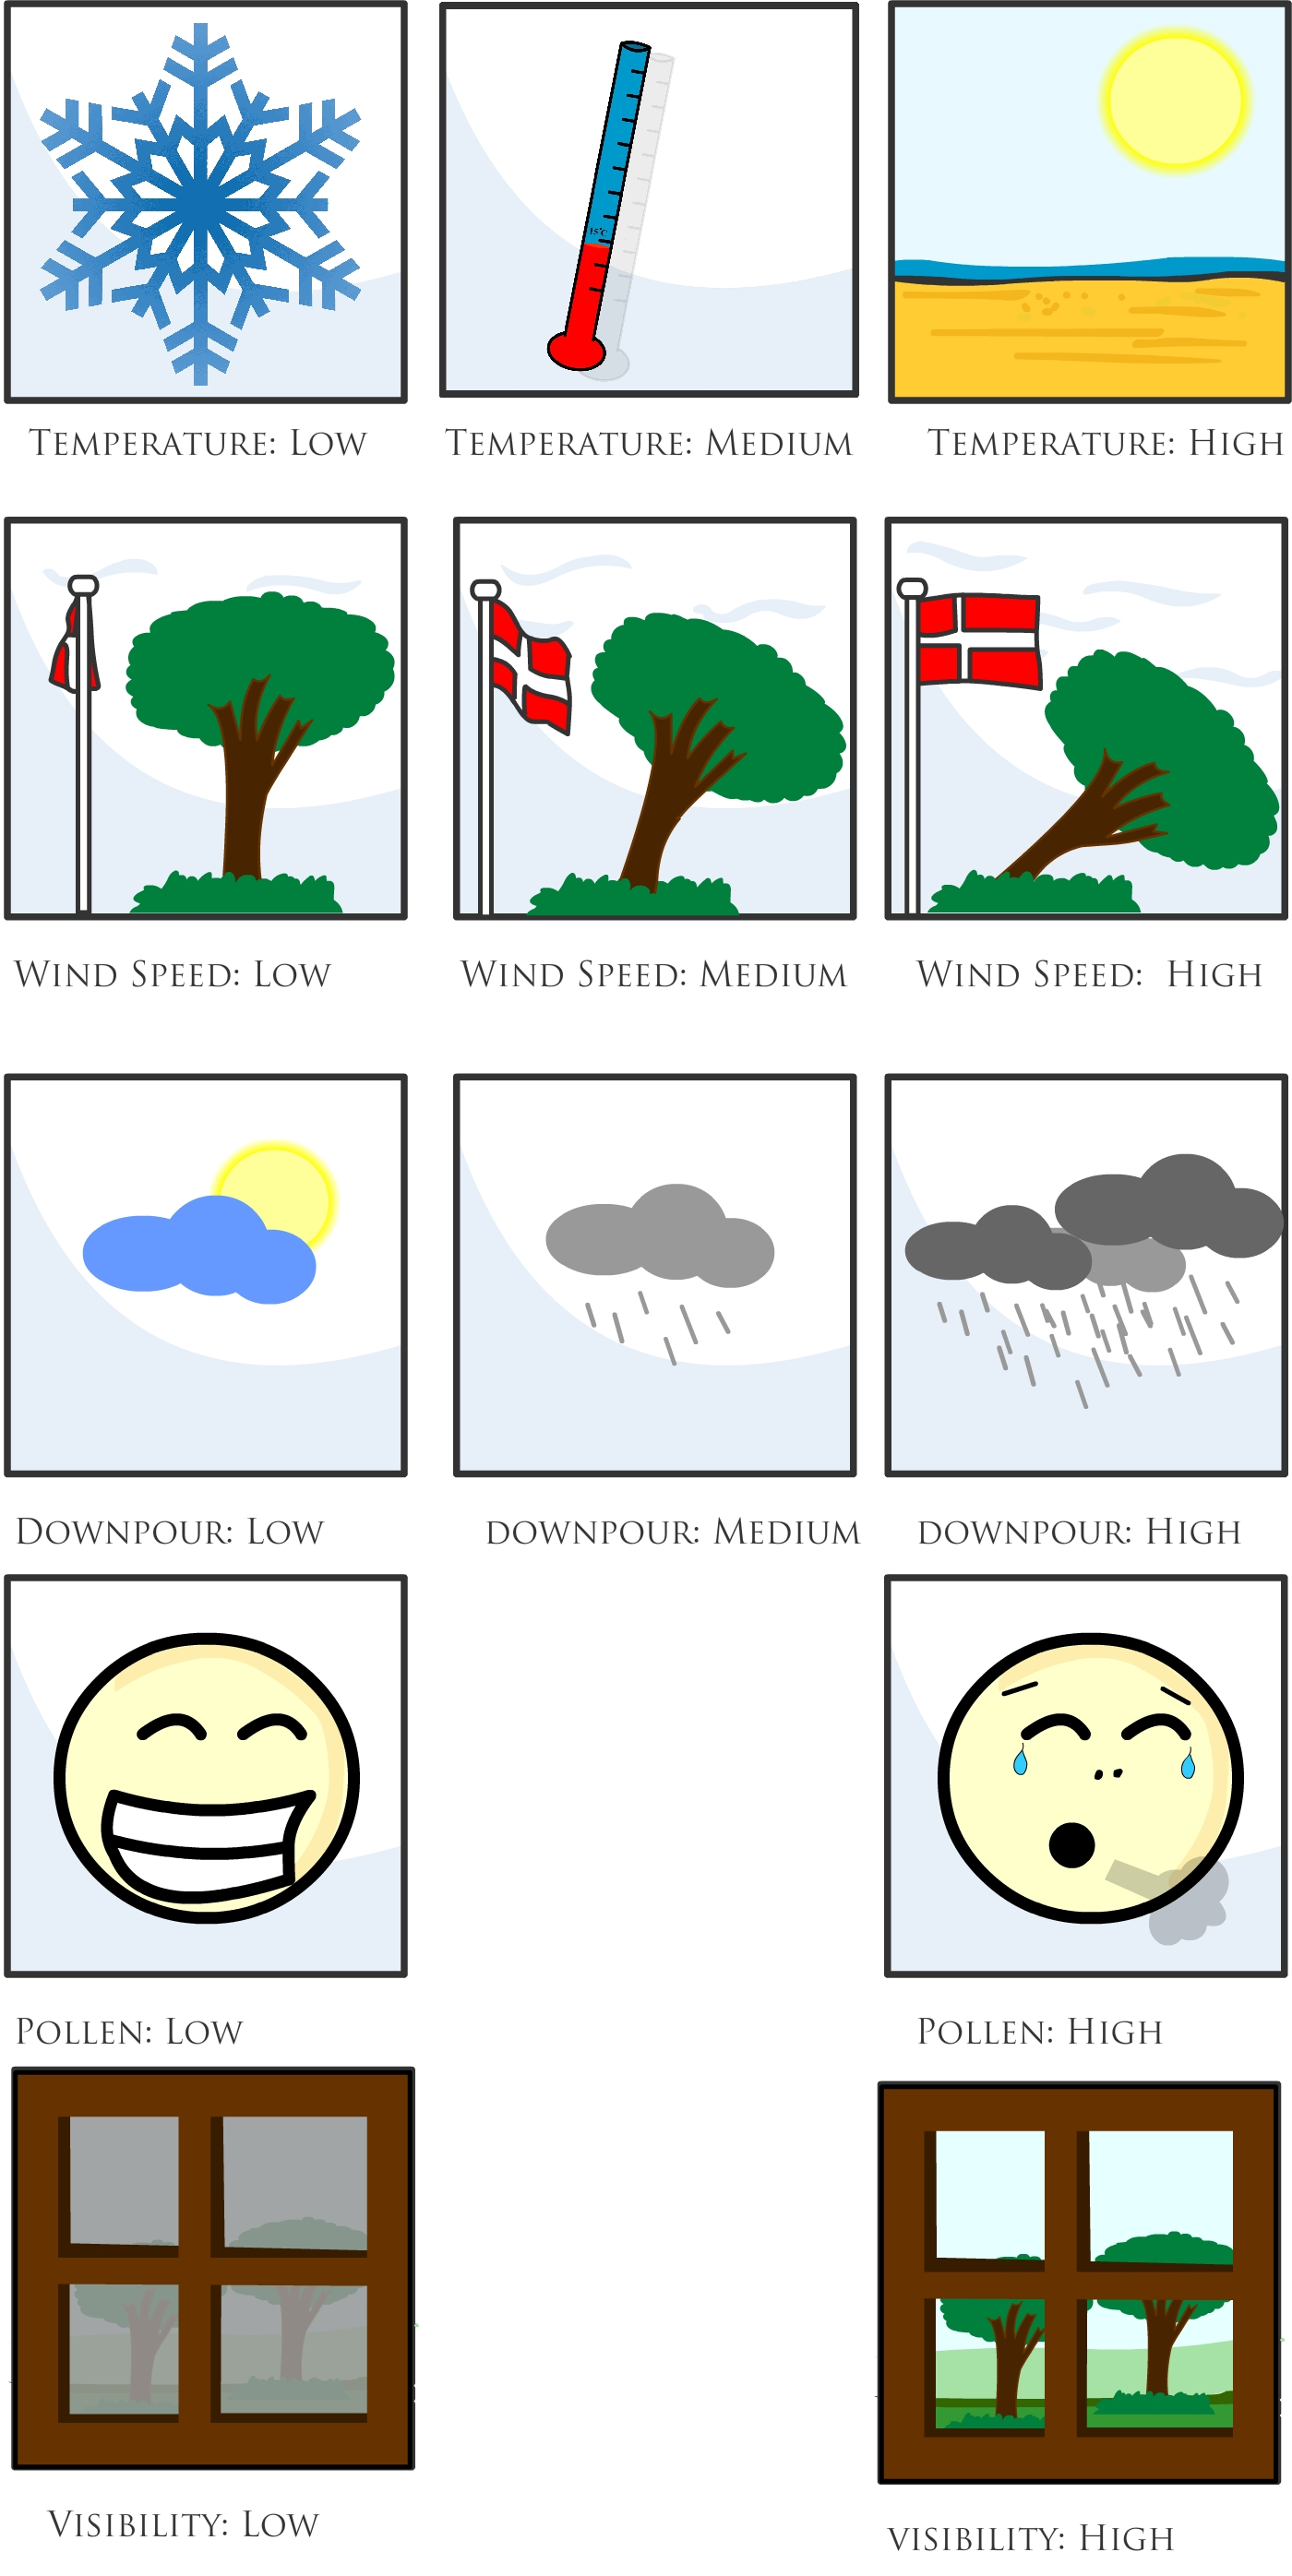
\includegraphics[width=0.7\textwidth]{images/Implementation11.jpg}
    \caption{Visual implementation}
    \label{fig:implementation11}
\end{figure}


% subsection visual_implementation (end)

\FloatBarrier
\subsection{Sound Implementation} % (fold)
\label{sub:sound_implementation}

As presented in the design (See section~\ref{ssub:how_the_sound_will_be_implemented_in_pure_data}), the following list is defined as the procedure of the implementation of the sounds in PureData.

\begin{enumerate}
    \item Input Sound
    \item Array / Sample
    \item Determine Sample Speed
    \item Phasor
    \item Merge Array and Sample Speed
    \item Fliter (if required)
    \item Output Sound
    \item Tracker
\end{enumerate}

Here is a overview of one of the pure data systems that has been made:

\begin{figure}[!htbp]
    \centering
    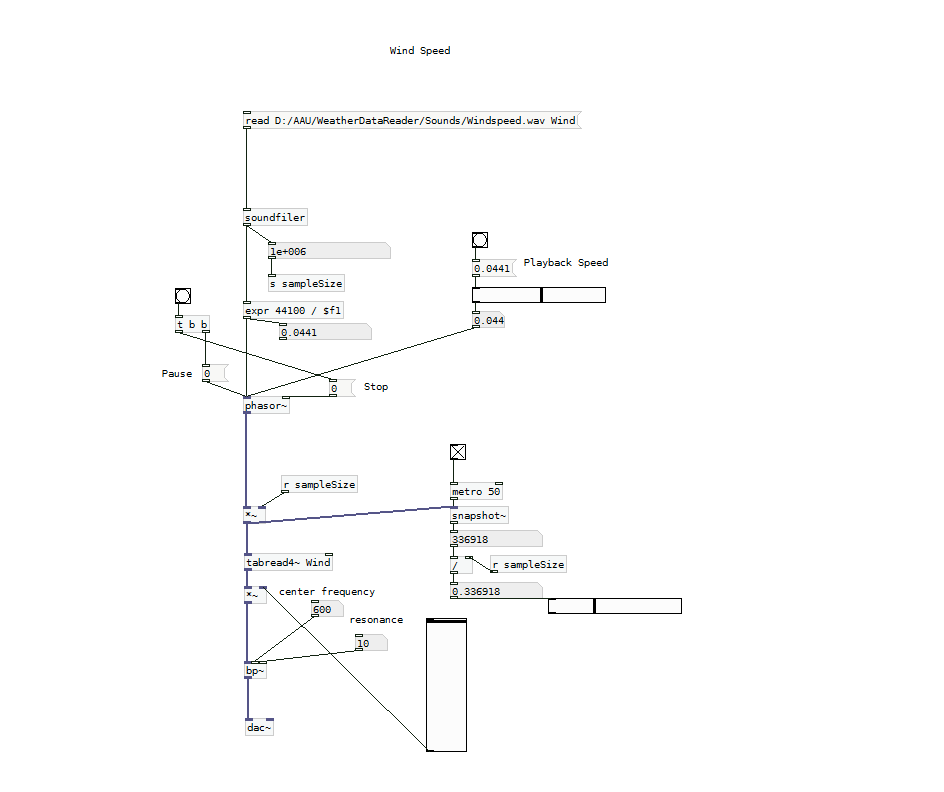
\includegraphics[width=1\textwidth]{images/Implementation1.png}
    \caption{Sample Pure Data implementation}
    \label{fig:implementation1}
\end{figure}

\FloatBarrier
\subsubsection*{Step 1} % (fold)
\label{ssub:step_1}

Here the program reads where the sound is placed on the computer and imports it into an array. 
As seen on the figure~\ref*{fig:implementation2} the path have been written down and in this case the array is called Wind.

\begin{figure}[!htbp]
    \centering
    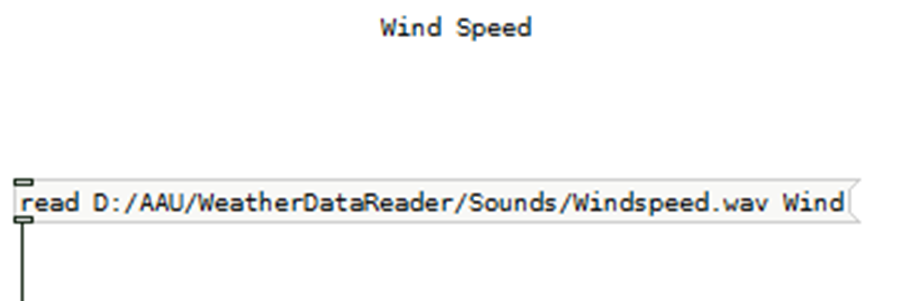
\includegraphics[width=.7\textwidth]{images/Implementation2.png}
    \caption{Sample audio import}
    \label{fig:implementation2}
\end{figure}

This is the array itself (Figure~\ref{fig:implementation3}). 
Here you can see what the different sound waves are going to look like. 
It might seem when you look at the arrays that there is a lot of wasted space in the array. 
This is simply because some of the sound don’t last that long and the empty space you see in the array is less than a second when played.

\begin{figure}[!htbp]
    \centering
    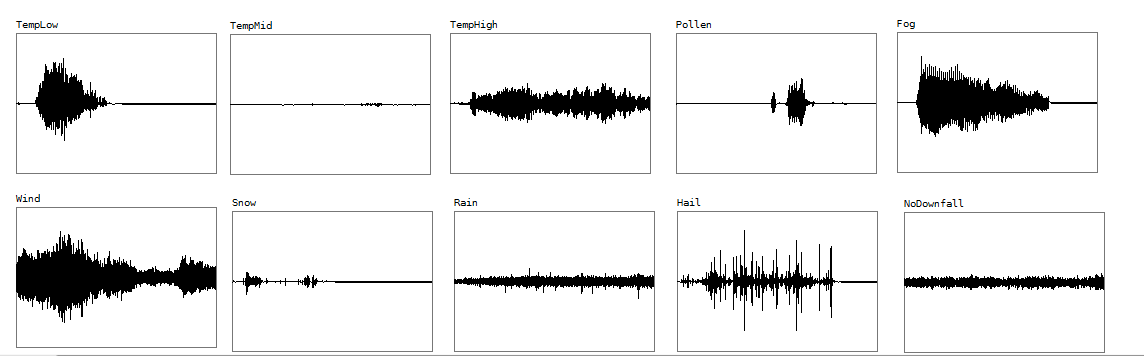
\includegraphics[width=.5\textwidth]{images/Implementation3.png}
    \caption{Sound sample array}
    \label{fig:implementation3}
\end{figure}

% subsubsection step_1 (end)

\FloatBarrier
\subsubsection*{Step 2} % (fold)
\label{ssub:step_2}

Here the soundfiler re-writes our floating points in the array to a binary sound file. 
As seen on the picture (Figure~\ref{fig:implementation4}) the sample amount is been read and stored in sampleSize which will be used later in the program to tell how big the array is. 
The samples then goes through a sampling that divides 44100 HZ with our sample size. This gives us the normal frequency. The data follows the path down to the phasor.

\begin{figure}[!htbp]
    \centering
    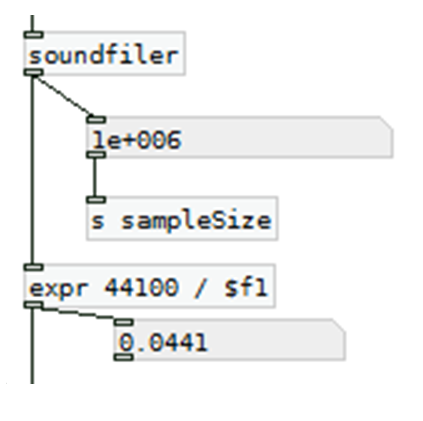
\includegraphics[width=.3\textwidth]{images/Implementation4.png}
    \caption{Soundfiler implementation}
    \label{fig:implementation4}
\end{figure}

% subsubsection step_2 (end)

\FloatBarrier
\subsubsection*{Step 3} % (fold)
\label{ssub:step_3}

We made a system that can control the speed of the samples. 
Using this, we can replace the original speed with our own to change the playback speed of the sound. 
This is using the custom made slider right besides the text Playback Speed on the picture (Figure~\ref{fig:implementation5}).

\begin{figure}[!htbp]
    \centering
    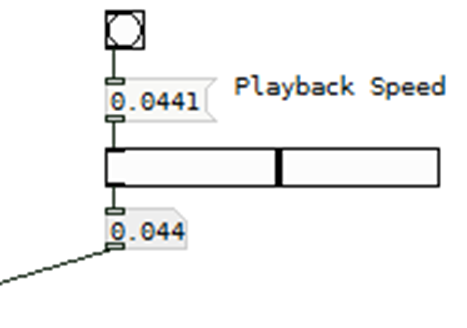
\includegraphics[width=0.3\textwidth]{images/Implementation5.png}
    \caption{Playback speep sample}
    \label{fig:implementation5}
\end{figure}

% subsubsection step_3 (end)

\FloatBarrier
\subsubsection*{Step 4} % (fold)
\label{ssub:step_4}

All the information sent to the phasor is now being used. The phasor detects a value between 1 and -1 to adjust the play speed. If the value is being set to 0 the waves in the phasor will be equal and stop the sound.
\begin{figure}[!htbp]
    \centering
    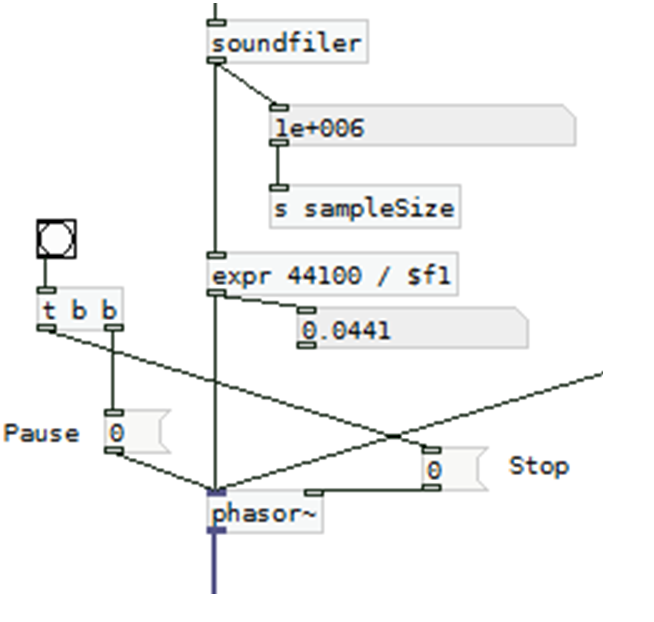
\includegraphics[width=0.3\textwidth]{images/Implementation6.png}
    \caption{Phasor}
    \label{fig:implementation6}
\end{figure}

% subsubsection step_4 (end)

\FloatBarrier
\subsubsection*{Step 5} % (fold)
\label{ssub:step_5}

Here (Figure~\ref{fig:implementation7}) 
The information from the phasor is being send into a binary signal operator that is being given a argument that is sampleSize. By doing this our progam now remembers how many samples there used to be. The samples can now merge with the array and tell what sample to move along further in the program.

\begin{figure}[!htbp]
    \centering
    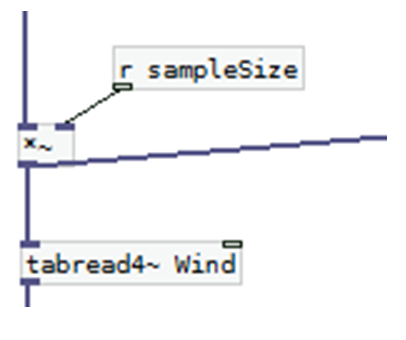
\includegraphics[width=0.3\textwidth]{images/Implementation7.png}
    \caption{Load old array}
    \label{fig:implementation7}
\end{figure}

% subsubsection step_5 (end)


\subsubsection*{Step 6} % (fold)
\label{ssub:step_6}

This is our bp filter as seen the two boxes linked to the filter are the center frequency and the resonance. 
In this case the center frequency is 600 and the resonance is 10.

\begin{figure}[!htbp]
    \centering
    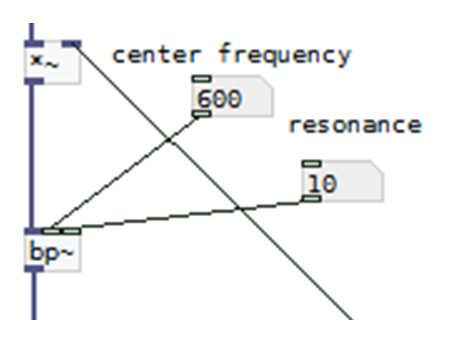
\includegraphics[width=0.3\textwidth]{images/Implementation8.png}
    \caption{bp Fliter}
    \label{fig:implementation8}
\end{figure}

% subsubsection step_6 (end)

\FloatBarrier
\subsubsection*{Step 7} % (fold)
\label{ssub:step_7}

After the filter all the information is sent to dac which is the audio output.

\begin{figure}[!htbp]
    \centering
    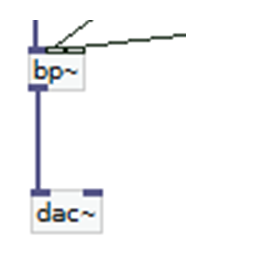
\includegraphics[width=0.2\textwidth]{images/Implementation9.png}
    \caption{dac output}
    \label{fig:implementation9}
\end{figure}

% subsubsection step_7 (end)

\FloatBarrier
\subsubsection*{Step 8} % (fold)
\label{ssub:step_8}

Additional feature:

A length tracker was implemented in order to know when the sound clip was done playing. This is done by tracking the samples going through the program.
This doesn’t change the sound output in any way but it’s useful to know during testing.

\begin{figure}[!htbp]
    \centering
    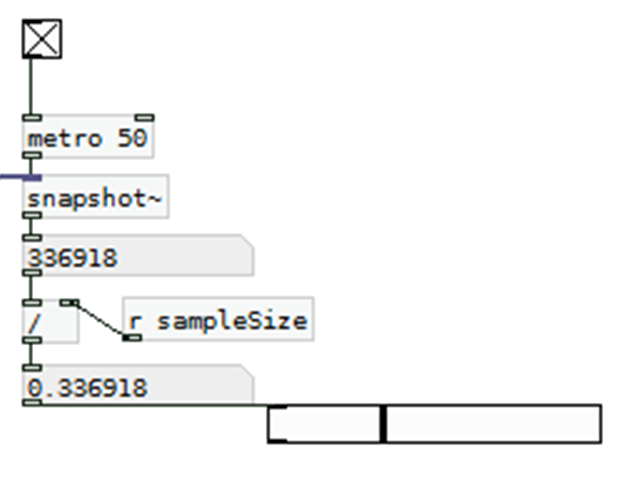
\includegraphics[width=0.3\textwidth]{images/Implementation10.png}
    \caption{Length Tracker}
    \label{fig:implementation10}
\end{figure}

\FloatBarrier
% subsubsection step_8 (end)

The rest of the sounds follow the same steps but the values is being replaced with these on our data sheet~\ref{tab:data_sheet}.

\begin{table}[!ht]
\centering
\begin{tabular}{l | l | l}
 & Play Speed & BP-Filter \\
\hline
Pollen & High: 0.418208 & N/A \\
\hline
Visibility & Low: 0.382 & N/A \\
\hline
Temperature & \specialcell{Low: 0.8339 \\ Mid: 0.0441 \\ High: 0.0882} & N/A \\
\hline
Downpour & \specialcell{Low: 0.06 \\ Mid: 0.2205 \\ High: 0.37} & N/A \\
\hline
Wind Speed & \specialcell{Low: 0.0441 \\ Mid: 0.0441 \\ High: 0.0441} & \specialcell{Low: 300 - 10 \\ Mid: 600 - 10 \\ high: 900 - 10}
\end{tabular}
\caption{Data sheet}
\label{tab:data_sheet}
\end{table}

Now that the sounds have been implemented the product is ready for testing. 
This leads us into the next step in the process, the evaluation of our prototype.
% subsection sound_implementation (end)

% section implementation (end)
%!TEX root = ../main.tex

\section{Evaluation} % (fold)
\label{sec:evaluation}

The evaluation will be divided into three separate test scenarios. 
As we are looking into how we can convey weather data through sonification, and how intuitively understood this information compared to visual representations of similar data is. 
It will be possible to evaluate upon by isolating and comparing data from several tests, where one test is of the produced sonifications, another test with visual elements and one test where both visuals and sonifications is tested.

More specifically described, a test will be conducted solely where the weather sonifications are presented to test subjects. 
Similarly, a test will be conducted where the visual representations will be presented with the same procedure as the sonification, and finally a test where both visual representations along with the sonification of the data.
This procedure will make it possible to compare what the test subjects can deduct from the presented data, and allow us to make comparisons towards what information the visual, sonification and combined representations of data is conveying, and thereby make it possible to evaluate upon how well the sonification formulate weather data.


\subsection{Method} % (fold)
\label{sub:method}

The primary reason of the evaluation is to establish knowledge to determine if the list of requirements has been fulfilled and to make it possible to gain satisfying results, which help answer the final problem statement.

The implemented prototype contains sonifications of specific weather categories, where these categories have been further categorised into sonifications of different values, which represent low, medium and high values of a specific weather category.

A Kruskal-Wallis test will be conducted on the gathered test results, which will be divided into three separate tests. 
This will ensure that it is possible to distinguish between the results gathered from the low values, medium values and the high values of the weather data, and will provide 3 separate box plots and associated data, which will allow us to prove or disprove the null hypothesis and to make assumptions and further analysis, which will help to answer the final problem statement.


\subsection{Procedure} % (fold)
\label{sub:procedure}

Here is the procedure for the test explained in detail. 
This chapter will describe the different aspects of the test such as sampling, observations, and guidelines for the testing. 
The same test procedure will be done on three separate presentations of weather conditions: visual presentation, audial representation, and combined presentation.
The general data for the tests are presented below.

Amount of participants: 20 subjects per category, per representation.
Test subject sampling: Convenience sampling: Aalborg university students.
Estimated length of test: 1 minute per subject.
Test location: Area on and around Aalborg university.
Date and time: When appropriate.


\subsubsection{Test setup} % (fold)
\label{ssub:test_setup}

The test will not require any specific location. 
For the testing only two people are present, i.e. 1 test subject and the test conductor. 
Only the combined test required two conductors for convenience purposes. 
The test subject and observer will be placed opposite each other during the test.
Other individuals, in this case other test subjects, will be placed out of view to avoid bias by previous subjects answers. 

% subsubsection test_setup (end)


\subsubsection*{Test Materials} % (fold)
\label{ssub:test_materials}
A listing of required materials for each test.

\paragraph{Visual test} % (fold)
\label{par:visual_test}

\begin{itemize}
    \item Visual samples: A set of images each representing a separate weather condition. The samples will be presented to the subject one at a time to avoid that the subject makes assumptions based on the other samples. 
    \item Notation sheets: Sheets of paper where the presented samples and respective responses are recorded.
\end{itemize}
% paragraph visual_test (end)

\paragraph{Sound test} % (fold)
\label{par:sound_test}

\begin{itemize}
    \item Audio samples: A set of audio snippets each representing a separate weather condition. The samples will be produced on scene using Pure Data and will not be prerecorded.
    \item Notation sheets: Sheets of paper where the presented samples and respective responses are recorded.
\end{itemize}
% paragraph sound_test (end)

\paragraph{Combined test} % (fold)
\label{par:combined_test}

\begin{itemize}
    \item Visual samples: The same samples from the visual test.
    \item Audio samples: the same samples from the audial test.
    \item Notation sheets.
\end{itemize}
% paragraph combined_test (end)

% subsubsection test_materials (end)


\subsubsection{Test Execution} % (fold)
\label{ssub:test_execution}

The testing procedure differs slightly in the three tests. 
In the visual test the subject is presented an image of a weather condition. 
The images do not contain the actual weather data they try to represent. 
During the audio test the subject is presented with an audio sample produced in Pure Data, and in the combined test the subject is presented with both an image and an audio sample of the same weather condition. 

The overall testing execution looks like this:

\begin{itemize}
    \item The subject is placed opposite the observer.
    \item The observer presents the subject with a sample.
    \item The presented sample is noted by the observer and the observer asks the subject if the sample presents a low, medium, or high value.
    \item The observer notes the answer and continues to the next sample until a sample from each category has been answered.
\end{itemize}
Before each test the subjects are informed that they are to be presented with 5 different samples (one for each category). 
They will be asked a question to each sample and that they are only to answer \enquote{high}, \enquote{medium}, or \enquote{low} to the questions. 
In order to ensure that each subject has the same understanding of the samples, they are given some context for each sample. 
This is done through the question asked to each sample. 
The question contains the weather condition but not the actual data i.e. \enquote{How much wind is in this image, high, medium, or low?} in case of a visual sample.
The subject will not be given any further clarification as we are looking for the intuitive guess and not the qualified guess.

% subsubsection test_execution (end)


\subsection{Hypothesis} % (fold)
\label{sub:hypothesis}

Based on the formulation of the final problem statement, the scientific experiment can be divided into two separate hypotheses. 
One hypothesis which specifies that there are no significant difference between the samples, and one hypothesis which specifies that there is some significant difference between the samples.


\subsubsection*{Null Hypothesis} % (fold)
\label{ssub:null_hypothesis}

There is no significant difference between the understanding of the non-speech auditory display of weather data using sonification techniques, compared to the understanding of visually presented weather information. 
% subsubsection null_hypothesis (end)

\subsubsection*{Alternative Hypothesis} % (fold)
\label{ssub:alternative_hypothesis}

There is some significant difference between the understanding of the non-speech auditory display of weather data using sonification techniques, compared to the understanding of visually presented weather information.

% subsubsection alternative_hypothesis (end)

\subsection{Test Delimitation} % (fold)
\label{sub:test_delimitation}

In order to prove or disprove the Null hypothesis, a statistical test is specified. 
The method of establishing what test will be used, the structure from Andy Field \& Graham Hole is utilized~\Cite[Ch. 8]{Field2003}.

\subsubsection{Type of data that is collected} % (fold)
\label{ssub:type_of_data_that_is_collected}

The data that is collected from the test participants is considered scores. 
As we are collecting data through a scientific study, the data that is contributed from the test participants are nominal data, being data that uses numbers to define categories or range of values which the test subjects think is correct.

What is obtained from the test participants is a value from 1-3 indicating low, medium or high values of a specific weather condition, which indicates their intuitive thought of what the formulated weather data represents.

% subsubsection type_of_data_that_is_collected (end)

\subsubsection{Independent variables} % (fold)
\label{ssub:independent_variables}

Independent variables, being something that is manipulated by us, is the weather conditions. 
There are one independent variable in this study, being the specific formulation of a single weather condition. 
As an example, the test subjects are presented with low/little rain as a visual image. 
Other test subjects are also presented with low/little rain, but as a sonification, or both. 
Then the test subjects provide scores, indicating what they actually think is presented.

% subsubsection independent_variables (end)

\subsubsection{Experiment design} % (fold)
\label{ssub:experiment_design}

As we are looking for differences or similarities between groups of people where we have altered independent variables, an experimental design is utilized.

% subsubsection experiment_design (end)

\subsubsection{Independent measures} % (fold)
\label{ssub:independent_measures}

Since we look for intuitively understood sonification of weather data, each participant will only be subjected to one condition of the test. 
This will allow us to obtain a single score from each participant in either the sonification, visual, or sonification \& visual test. The study can therefore be described as a wholly independent measure designed test.

The test subjects will be allowed to contribute with several answers within the same condition, but will not be allowed to contribute to others.

% subsubsection independent_measures (end)

\subsubsection{Non-parametric} % (fold)
\label{ssub:non_parametric}

As we have no pre-defined assumptions to the test, and to what extent there might be certain characteristics, the study can be described as non-parametric.

% subsubsection non_parametric (end)

\subsubsection{Test groups} % (fold)
\label{ssub:test_groups}

As specified as the independent variable, there are three different groups which will contribute with scores.

% subsubsection test_groups (end)

\subsubsection{Kruskal-Wallis Test} % (fold)
\label{ssub:kruskal_wallis_test}

By delimitating the above mentioned steps, it is defined that a Kruskal-Wallis test can be utilized to prove or disprove the Null hypothesis.


A Kruskal-Wallis test compares between the medians of two or more samples, to determine if the samples have come from different populations. 
This will make it possible to know if the samples are similar or different, given the independent variable and can tell us if the test subjects understand visual, auditory or both in different or similar manners, and the actual distribution of data~\cite{Gaten2000}.


There are however, some limitations to the Kruskal-Wallis test.
If no significant difference in our data is found, the samples can not be concluded as to being similar.
If there are any significant differences, it is not possible to make specific assumptions as to what contributed to the significant difference. 
Further analysis and testing would be required. \cite*{Gaten2000}.
% subsubsection kruskal_wallis_test (end)

% subsubsection test_delimitation (end)

% subsection hypothesis (end)

% subsection procedure (end)

% subsection method (end)

\subsection{Results} % (fold)
\label{sub:results}

The results from the test are here presented and described. 
Discussions and interpretations of the results are conducted in the Evaluation: Discussion (Section~\ref{sub:discussion})

The gathered results can be found in appendix~\ref{sec:test_results}.

\begin{figure}[!htbp]
    \centering
    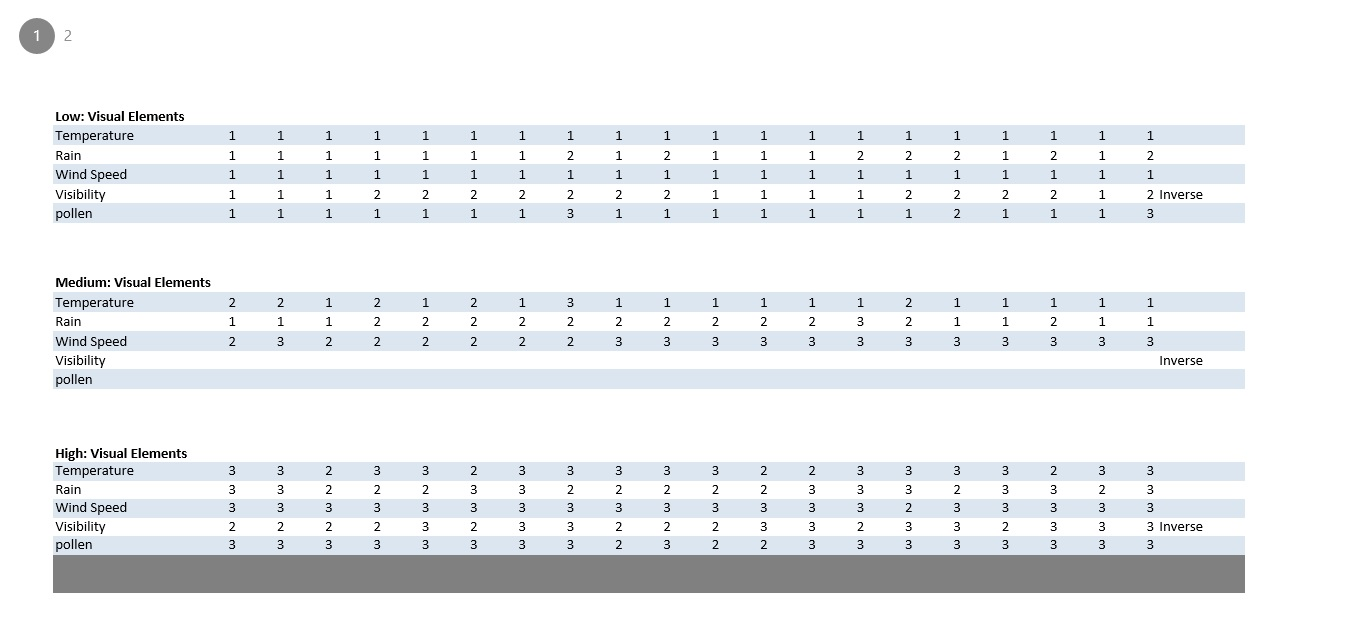
\includegraphics[width=1\textwidth]{images/Evaluation1.jpg}
    \caption{Test result snippet}
    \label{fig:evaluation1}
\end{figure}

As seen on figure~\ref{fig:evaluation1}, there are three categories. 
Low elements, medium elements, and high elements. 
This example only covers the visual weather data. 
The results gathered from Sonification, and sonification \& Visual elements can be found in the appendix~\ref{sec:test_results}.

The numbers indicates the responses from 20 test participants. 
These are labels of 1-2-3 which indicates low, medium and high values.

The rows indicates responses from a single test participant.

\begin{itemize}
    \item Low values has the label: 1
    \item Medium values has the label: 2
    \item High values has the label: 3
\end{itemize}

The \enquote{inverse} represents that the data from the specific data set has been inversed. 
As visibility had the correct answer of 3, but as the labelling indicates, the low value label is 1, therefore to make the responses match the other results, the data is inverted. 
This way, it is possible to know that each response of 1 is correct or opposite.


It can be deduced from figure~\ref{fig:evaluation1}, that if a low weather condition has been answered and labeled with 1, then the answer is correct, as the image illustrates a weather condition of low value. 
Likewise with medium values which has the answer 2 and high values with an answer of 3. 
If a medium sound is heard, and the test subject answers correctly with a response of medium, then 2 is noted.

\subsection{Kruskal-Wallis Test Results} % (fold)
\label{sub:kruskal_wallis_test_results}

The test results will be divided into three separate Kruskal-Wallis tests, in order to evaluate upon low data, medium data and high data separately, to make the distinction between the independent variable more clearly. 
The outcome is a Boxplot, respectively of low, medium and high weather data elements along with the data descriptions of the three Kruskal-Wallis tests.


\subsubsection*{Low values: Kruskal-Wallis ANOVA table} % (fold)
\label{ssub:low_values_kruskal_wallis_anova_table}

\begin{figure}[!htbp]
    \centering
    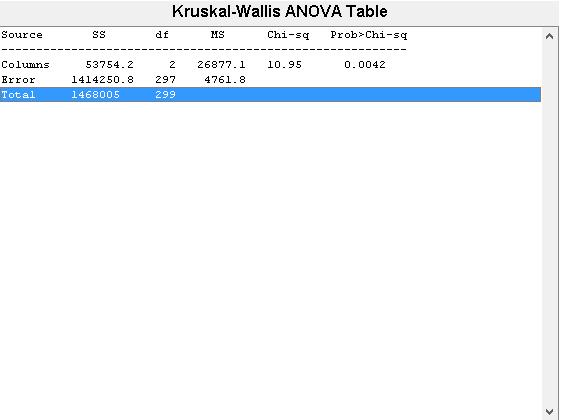
\includegraphics[width=.7\textwidth]{images/Evaluation2.jpg}
    \caption{ANOVA table low data}
    \label{fig:evaluation2}
\end{figure}

The P value(Prob>Chi-sq) is 0.0042 which is under 0.05. 
Therefore the null hypothesis is rejected and accepts the alternative hypothesis.

This means that we accept that there is some significant difference between the understanding of the non-speech auditory display of weather data using sonification techniques, compared to the understanding of visually presented weather information, specifically for low value data, which has been specified as the alternative hypothesis.

% subsubsection low_values_kruskal_wallis_anova_table (end)

\FloatBarrier
\subsubsection*{Low values: Kruskal-Wallis test results} % (fold)
\label{ssub:low_values_kruskal_wallis_test_results}

\begin{figure}[!htbp]
    \centering
    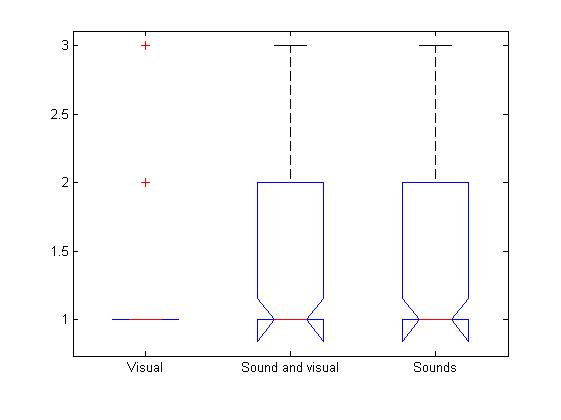
\includegraphics[width=.5\textwidth]{images/Evaluation3.jpg}
    \caption{Boxplot low data}
    \label{fig:evaluation3}
\end{figure}

Generally the boxplot indicates similar levels of medians but the visual scale has a different distribution than \enquote{Sound and Visual} and \enquote{Sounds}.

The \enquote{Visual} element is comparatively short, as the inner quartile range is overlapping, which suggests that a high number of responses are 1. 
A majority of participants answered correctly, but a low number of participants, indicated by the \enquote{plus}, that 2 and 3 was also answered by a lower population of the test participants.

% subsubsection low_values_kruskal_wallis_test_results (end)

\FloatBarrier
\subsubsection*{Medium values: Kruskal-Wallis ANOVA-Table} % (fold)
\label{ssub:medium_values_kruskal_wallis_anova_table}

\begin{figure}[!htbp]
    \centering
    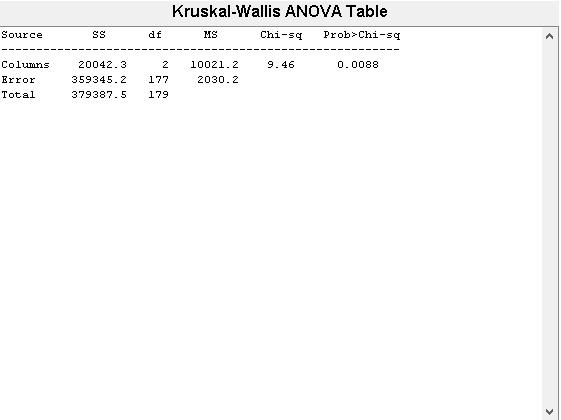
\includegraphics[width=0.7\textwidth]{images/Evaluation5.jpg}
    \caption{ANOVA table medium data}
    \label{fig:evaluation5}
\end{figure}

As seen on figure \ref{fig:evaluation5} the P value (Prob>Chi-sq) is 0.0088 and is therefore below the confidence interval of 0.05 and does therefore disprove the Null hypothesis and accept the alternative hypothesis.

% subsubsection medium_values_kruskal_wallis_anova_table (end)

\FloatBarrier
\subsubsection*{Medium values: Kruskal-Wallis Boxplot results} % (fold)
\label{ssub:medium_values_kruskal_wallis_boxplot_results}

\begin{figure}[!htbp]
    \centering
    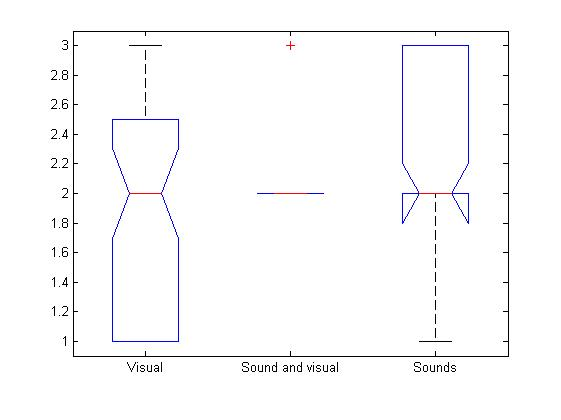
\includegraphics[width=.7\textwidth]{images/Evaluation7.jpg}
    \caption{Boxplot medium data}
    \label{fig:evaluation7}
\end{figure}

The Boxplot of the medium values, see figure \ref{fig:evaluation7}, illustrates the distribution of the test results amongst the acquired data. The median of the three data samples are generally similar, but the distribution of responses are somewhat different. 
The median amongst the samples are 2, which is also the label which represents middle value data.

The \enquote{Visual} boxplot indicates a minimum value which collides with the lower quartile and describes that atleast 50 percent of the test participants has answered 1 in the visual test of medium values. 
Another 25 percent has answered 2, and the maximum value indicates that 25 percent has answered 3, which is labelled as the high value.

The \enquote{Sound and Visual} illustrates, as the upper and lower quartiles, along with the maximum and minimum is overlapping, illustrates that a majority of the test participants has answered 2, being the correct answer. 
Only a few test participants has answered 3 which is the label of high values.

Lastly, the \enquote{Sound} being the sonification of the medium valued weather data indicates that the median is 2, with a upper quartile of 25 percent having answered 3, along with 50 percent having answered 1.

% subsubsection medium_values_kruskal_wallis_boxplot_results (end)

\FloatBarrier
\subsubsection*{High values: Kruskal-Wallis ANOVA-Table} % (fold)
\label{ssub:high_values_kruskal_wallis_anova_table}

\begin{figure}[!htbp]
    \centering
    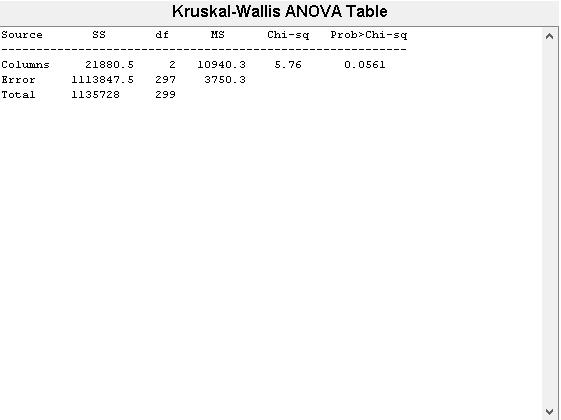
\includegraphics[width=0.7\textwidth]{images/Evaluation6.jpg}
    \caption{ANOVA table high data}
    \label{fig:evaluation6}
\end{figure}

The P. value (Prob>Chi-sq) is 0.0561 and is above 0.05 then indicates that we fail to reject the null hypothesis with specifically high value weather condition results.

Therefore here is no significant difference between the understanding of the non-speech auditory display of weather data using sonification techniques, compared to the understanding of visually presented weather information specifically for high value weather conditions.

% subsubsection high_values_kruskal_wallis_anova_table (end)

\FloatBarrier
\subsubsection*{High values: Kruskal-Wallis Boxplot results} % (fold)
\label{ssub:high_values_kruskal_wallis_boxplot_results}

\begin{figure}[!htbp]
    \centering
    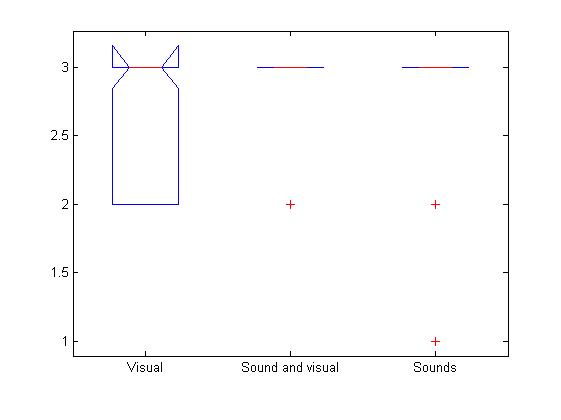
\includegraphics[width=.7\textwidth]{images/Evaluation8.jpg}
    \caption{Boxplot high data}
    \label{fig:evaluation8}
\end{figure}

The High-value boxplot of which the null hypothesis is accepted, there are no significant difference in the samples. 
They are however not similar.
The Visual sample indicates that 25\% of the test subjects thought of some or more of the visual interpretations of weather conditions as being a middle value. 
There are however in the sound and visual sample below 25\% who thought that is was a medium value. 
And with the sound sample, below 25\% of the test participants thought that the sonification indicated either low or medium, leaving 75\% test participants answering correctly.

% subsubsection high_values_kruskal_wallis_boxplot_results (end)

% subsubsection kruskal_wallis_test_results (end)

\FloatBarrier
\subsubsection*{Graphical test results} % (fold)
\label{ssub:graphical_test_results}

As the Kruskal-Wallis test only provides knowledge of statistical differences of the data groups, it is also important to gain knowledge of the specific weather condition elements which proved to be successful or unsuccessful. 
In order to elaborate upon what sounds, compared to the visual elements had any/if any specific impact. 
Therefore a graphical structure of the results are developed (See appendix~\ref{sub:test_result_graphs}).

\begin{figure}[!htbp]
    \centering
    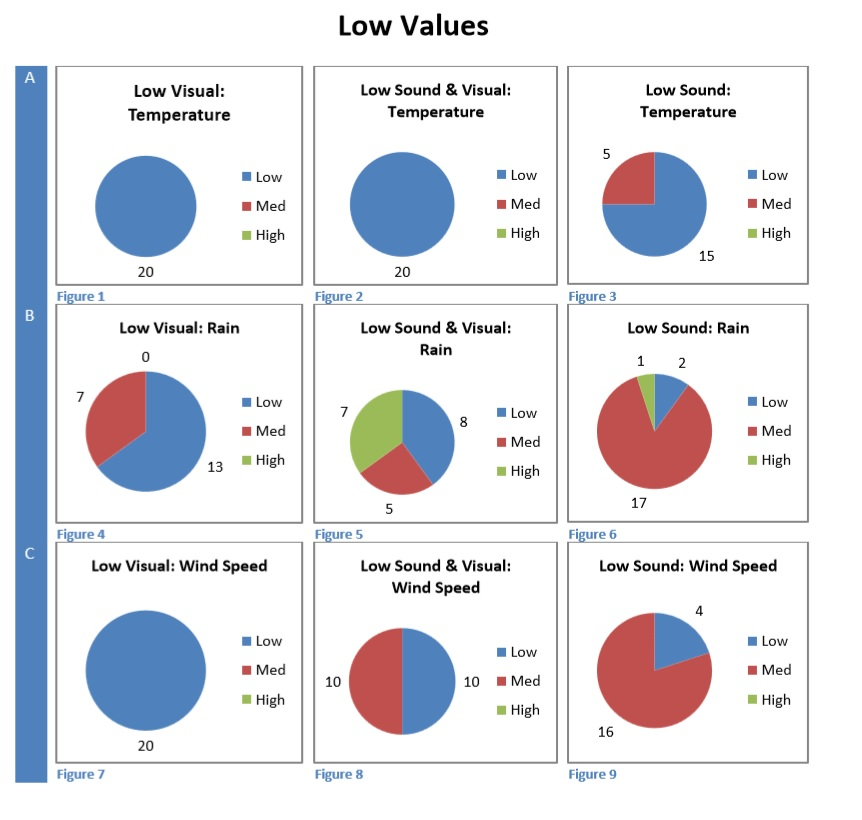
\includegraphics[width=.7\textwidth]{images/Evaluation4.jpg}
    \caption{Snippet of graphic chart: Test Results}
    \label{fig:evaluation4}
\end{figure}

As seen on figure~\ref{fig:evaluation4}, a snippet of the pie charts are presented. 
On the row A1-3, the three temperature results is comparable. 
The pie charts each represents 20 responses and indicates the participants answers of the visual elements, sound and visual elements and the sound element. 

Each pie chart illustrates the number of answers for low, medium and high which is illustrated by a percentage of the chart in a color and a number that indicates the amount of test participants who answered that specific value. 
The title refers to the sound that has been played to the test subjects.

% subsubsection graphical_test_results (end)

% subsection results (end)

\FloatBarrier
\subsection{Discussion} % (fold)
\label{sub:discussion}

Here, the discussion and interpretations of the results are presented. 
What is deducted from the data and what thoughts as towards what the answers indicate will be described and explained.

\subsubsection{Kruskal-Wallis tests Boxplots} % (fold)
\label{ssub:kruskal_wallis_tests_boxplots}

\paragraph{Low Value:} % (fold)
\label{par:low_value_}
\hspace{0pt} \\
The low value boxplot (Figure~\ref{fig:evaluation3_2}) compliments the ANOVA table and illustrates significant difference of the independent variables between the \enquote{visual}, the \enquote{sonification} and \enquote{both combined}, which is the altered independent variable.

We can see that a large amount of participants answered correctly on the visual test, but a few who answered two or three. 
Although the numbers are very few, it is not enough to increase the upper quartile, meaning that the ones who answered incorrectly are below 25\%.  
With the \enquote{sound} and \enquote{sound \& visual}, the upper quartile indicates that from the median up to maximum, 50\% of test participants answered incorrectly, as the correct answer was 1, being the label of low. 
A large amount of the test participants answered 2 (25\%) or 3 (25\%). 
This indicates that a large amount of the test participants misinterpreted the sonification of low weather conditions.

\begin{figure}[!htbp]
    \centering
    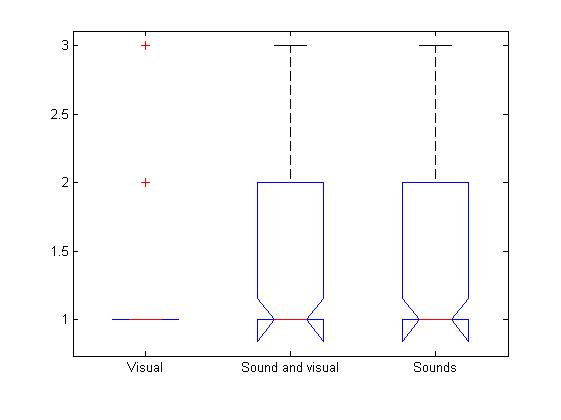
\includegraphics[width=.5\textwidth]{images/Evaluation3.jpg}
    \caption{Boxplot low data}
    \label{fig:evaluation3_2}
\end{figure}

% paragraph low_value_ (end)

\paragraph{Middle Value:} % (fold)
\label{par:middle_value_}
\hspace{0pt} \\
The middle value Boxplot (See figure \ref{fig:evaluation7_2}) indicates a difference in the \enquote{visual}, \enquote{sound} and \enquote{sound \& visual} test results, which also is indicated as the null hypothesis is accepted, and that we therefore conclude there there is a some significant difference between the understanding of the non-speech auditory display of weather data using sonification techniques, compared to the understanding of visually presented weather information.

On all three groups, the medians are 2, which is the correct label for the middle value, and illustrates that a majority of the test participants answered correctly in each of the three tests.

The notched boxplot \enquote{Visual} illustrates that 50\% of the test participants answered 1, which is incorrect and lower than the intended formulation. 
There are however below 25\% who answered incorrectly in the test where Sound \& Visual was presented, and only 3 (high value) was answered wrong by a small number of the test participants.

Lastly the boxplot for \enquote{Sound} indicate that a majority answered correctly with 2, but 25\% answered 3, and another percentage of test subjects answered 1, which indicates that there are a majority of test subjects that misinterpreted the middle value sonifications. 

\begin{figure}[!htbp]
    \centering
    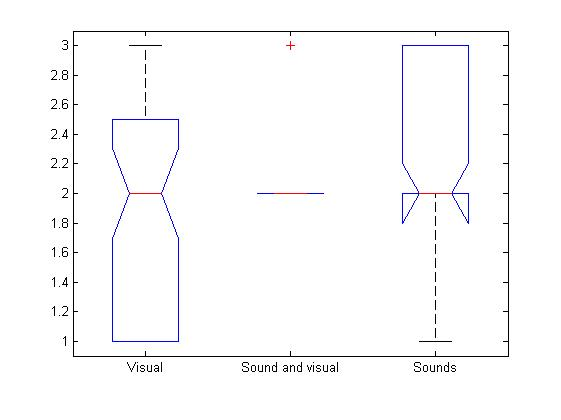
\includegraphics[width=.7\textwidth]{images/Evaluation7.jpg}
    \caption{Boxplot medium data}
    \label{fig:evaluation7_2}
\end{figure}

% paragraph middle_value_ (end)

\paragraph{High Value:} % (fold)
\label{par:high_value_}
\hspace{0pt} \\
The High-value boxplot of which the null hypothesis is accepted, there are no significant difference in the samples. 
They are however not similar.
The Visual sample indicates that 25\% of the test subjects thought of some or more of the visual interpretations of weather conditions as being a middle value. 
There are however in the sound and visual sample below 25\% who thought that is was a medium value. 
And with the sound sample, below 25\% of the test participants thought that the sonification indicated either low or medium, leaving 75\% test participants answering correctly.

\begin{figure}[!htbp]
    \centering
    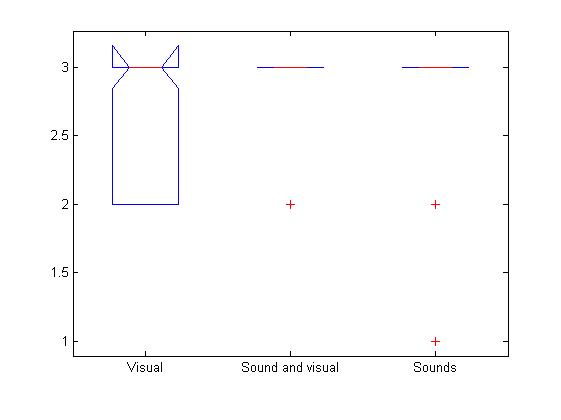
\includegraphics[width=.7\textwidth]{images/Evaluation8.jpg}
    \caption{Boxplot high data}
    \label{fig:evaluation8_2}
\end{figure}

% paragraph high_value_ (end)

% subsubsection kruskal_wallis_tests_boxplots (end)

\FloatBarrier
\subsection{Pie charts} % (fold)
\label{sub:pie_charts}
Although the boxplot and ANOVA tables indicates similarities or differences between the samples, they do not describe what specific sounds/visuals had any impact or what could have been done differently or what specific sounds were actually successful in conveyance of sonifications of weather data.

The following appendix~\ref{sub:test_result_graphs} indicates the numbers of correct/incorrect responses of each weather category, and makes it possible for comparisons.

Though it is possible with our test results to elaborate upon which sonifications were successfully implemented, and to which degree, it is not possible to make assumptions based upon acquired evidence what actually was a success, and what was incorrect in the implementation of the sonifications.

More specifically, it implies that we are able to observe the number of correct or incorrect responses from the test subjects, but we are unable to answer why we obtain these specific data sets based upon the acquired scientific test results.

As we are only able to make assumptions based upon the acquired data, this will be discussed in the following chapter (See discussion, section~\ref{sec:discussion}).

% subsection pie_charts (end)

% section evaluation (end)
\section{Re-design} \label{sec:redesign}
\lipsum[1]

%!TEX root = ../main.tex

\section{Discussion} % (fold)
\label{sec:discussion}

In this chapter the project will be discussed and reflected upon. 
This includes insight as to what could have been done differently to improve the acquired results, or and what impact any decision throughout the report might have had. 
Ultimately the discussion will lead to how the problem statement can be answered i.e. how well the problem was solved, and what this result implies.

For the visual part of our test, (See chapter \ref{sub:visual_pre_test}) we conducted the test using images created by ourselves, based upon the visual pre test, which could have changed/affected the test results. We chose to create our own pictures since we believed it would not matter if they were taken from a website or drawn by us. We based our drawings on information given from the visual pre-test . The test results indicates that not everyone could see what the pictures represented(See appendix \ref{sub:test_result_graphs}) This is of course an issue and for further testing these images should perhaps be replaced with something not based on our pre-test, but pictures found on weather represented websites or authored by a professional. Pictures as these may be more recognizable for people since there’s a chance they have seen them in weather forecasts on TV or in newspapers, which could in turn lead to different test results.


Something that might have made a difference to our test results is the implemented filters. 
The idea of changing some aspects in the sounds might not have worked out as well as we had hoped.
From our observations during testing, we observed that even though we changed some of the sound it still sounded the same for the testers. 
An example of this is that our rain sound might sound similar at the medium and high values. 
This is most likely because they never heard the other sounds for the two other values, so they had nothing to mentally compare with. It was also not possible to make it sound like there was close to no rain, without making it sound unnatural. We believe that it could be more efficient to have different sounds instead of changing one sound to represent the different weather data values.


In the design (See section \ref{ssub:categories} ) it was delimitated that the range of weather condition data should not be sonified in a continuous manner, where every value had a sonification, but rather in sections which were represented by low, medium, or high values in which the specific weather condition was implied which was described as event based sonifications. 
By making the decision of delimitating the amount of sonifications, and altering the sonifications from exact values to an indication of a specific range of values formulated by a label of low, medium, or high where the understanding is individual to each test subject, the sonification itself is altered to formulate another type of content, rather than the actual weather data. 

What this implies is that we make a predetermined decision towards the possibility of making an exact sonification of the entire ranges of values in a specific weather condition, and to be intuitively understandable, which we believe to be impossible.

The obtained test results have both positive and negative indications regarding the success of intuitively understanding the visual and sonified weather data, but the data only represents low, medium, and high values, where a continuous sonifications of weather data should indicate degrees, wind speed etc. where decimals are included, if it was to be an exact interpretation of the designated set of data. 

In the analysis chapter (See chapter \ref{ssub:weather_data_represented_using_sound} ), an example is provided where a similar procedure was used. In this example it is stated that engineers had to repeatedly listen to the different predefined values for a while, before being familiar enough with the sound to understand what it meant. This is unlike the intuitive sonifications which a user should be able to understand without having to learn what data the sonification implies.

The evaluation chapter in this report provides data from the test subjects that indicate differences or similarities in the data, when using the Kruskal-Wallis tests, and provides detailed information about specific weather condition data, which was correctly or incorrectly answered. See section (\ref{sub:results}) for evaluation results. However, there was not obtained test data, which elaborates upon why any of the presented weather data conditions were answered correctly or incorrectly, but we do have theories.


The pie charts (see appendix \ref{sub:test_result_graphs}) show the responses for each weather data information, indicated by a single pie chart in the appendix. The data does not specifically reflect the following , but we assume that weather conditions which actually have a sound are more likely to be intuitively understood than weather data which have no sound (but this is understood via associations). An example is Wind speed (See appendix \ref{sub:test_result_graphs}, K32). When there is wind, it is possible to hear the wind, unlike temperature. There is no sound of temperature, but associations that makes one think that there must be a specific temperature because of associated sounds. 100 percent of test participants answered correctly on high wind so a plausible solution can be that the sound is intuitive as there already exists specific sounds for wind. However, as indicated by low rain (Appendix \ref{sub:test_result_graphs},  B6), where there is a sound for low amount of rain, 17 out of 20 answered incorrectly even though rain ought to be intuitive much like wind speed. The reason for this error could however be our choice of sound representation which could indicate some other values. e.g. mid or high value of the data, leading the test subjects to answer incorrectly.

It can also be argued that associations to weather data is an individual interpretation, which makes it unlikely to make accurate sonifications of weather data, as there is no correct choice of sonifications to illustrate an association to the specific weather data, but only a plausible majority who may think that a specific sound/sonification accurately conveys that data.

While interpreting the results of the test, it became apparent that while it could be possible to evaluate upon each specific visualisation and sonification of the weather data, it would not result in any new information, which would allow for a more thorough and accurate answer to the final problem statement. This is because of the delimitation that has been made early in the design phase. The delimitation is the choice of only conducting sonifications of low, medium and high values. A re-design could be conducted where a questionnaire would be added to the predefined test structure where test subjects would be asked to describe what they think could be altered within the visualizations and sounds/sofications. This would give indications as to what could be altered in order to gain more accurate results, which would be reflected in the pie charts of each specific set of data values.

However, even if the test would be conducted and the sonifications and visualizations would be modified numerous times until the data from the tests would indicate that 100 percent of the test subjects answered correctly, the sonications are still delimited to low, medium and high values. 

For this very reason it would seem unimportant to conduct further testing and re-design of the product. We would gain evidence to support the claim that it is possible to intuitively convey weather data, if the data is limited to low, medium and high values, but the test results is already indicating such assumptions to some extend whereof a number of test participants are answering correctly on each of the sonifications.


With what we have discussed so far, we can begin to discuss answering the final problem statement.


"To what extent is it possible to convey weather information, solely as a nonspeech auditory display, using sonification techniques, and be as intuitively understandable as visually presented weather information, where intuitive is defined as knowing by intuition?"


“To what extent...” is as mentioned defined by the choice of delimiting the continuous weather data values to labels of low, medium and high. We can therefore argue that it is indeed possible to convey weather information, solely as a nonspeech auditory display, using sonifications techniques, where the conveyed data is weather conditions with low, medium and high values. 

The pretests (see chapter \ref{sub:visual_pre_test} and \ref{sub:sound_pre_test})  indicates specific visualisations and sounds which could be utilized to the sonification of the data, which supports that the conveyed data is intuitive, meaning that a majority of the test participants could relate and understand the specific weather condition along with the specified data value, being low, medium or high. Also, as the results indicate, only a limited number of test participants answered correctly, but we assume that a refined product would make it possible to gain more satisfactory results, obtaining results that indicate a high margin of correctly answered questions within the low, medium and high labeled values of each weather condition.

Lastly, as we have also delimited the weather information, we can only account for the specified weather conditions as mentioned.

To elaborate upon the possibility of making sonifications to represent continuous values of a weather condition, in addition to the labels of low, medium and high, would require further testing, but we deem it possible.However, we question the usability, as the difficulty of conveying such small differences and changes would be very high. It would be very difficult for a person to either understand intuitively, remember, or even learn it in the first place.


% section discussion (end)
\section{Conclusion} \label{sec:conclusion}
\lipsum[1]

\clearpage
%------------------------------------------------------------------------------
% BIBLIOGRAPHY
%------------------------------------------------------------------------------
\pagestyle{plain}
\label{bibliography}
\printbibliography[heading=bibintoc]

\clearpage
%------------------------------------------------------------------------------
% APPENDICES
%------------------------------------------------------------------------------
% once appendices are started we can't go back
% make sure this is the last include!!!
%!TEX root = ../main.tex

\appendix
\appendixpage
\addappheadtotoc
\noappendicestocpagenum

\section{Visual Pre-test} \label{sec:visual_pre_test_raw_results}
\subsection{Raw Results} % (fold)
\label{sub:raw_results}

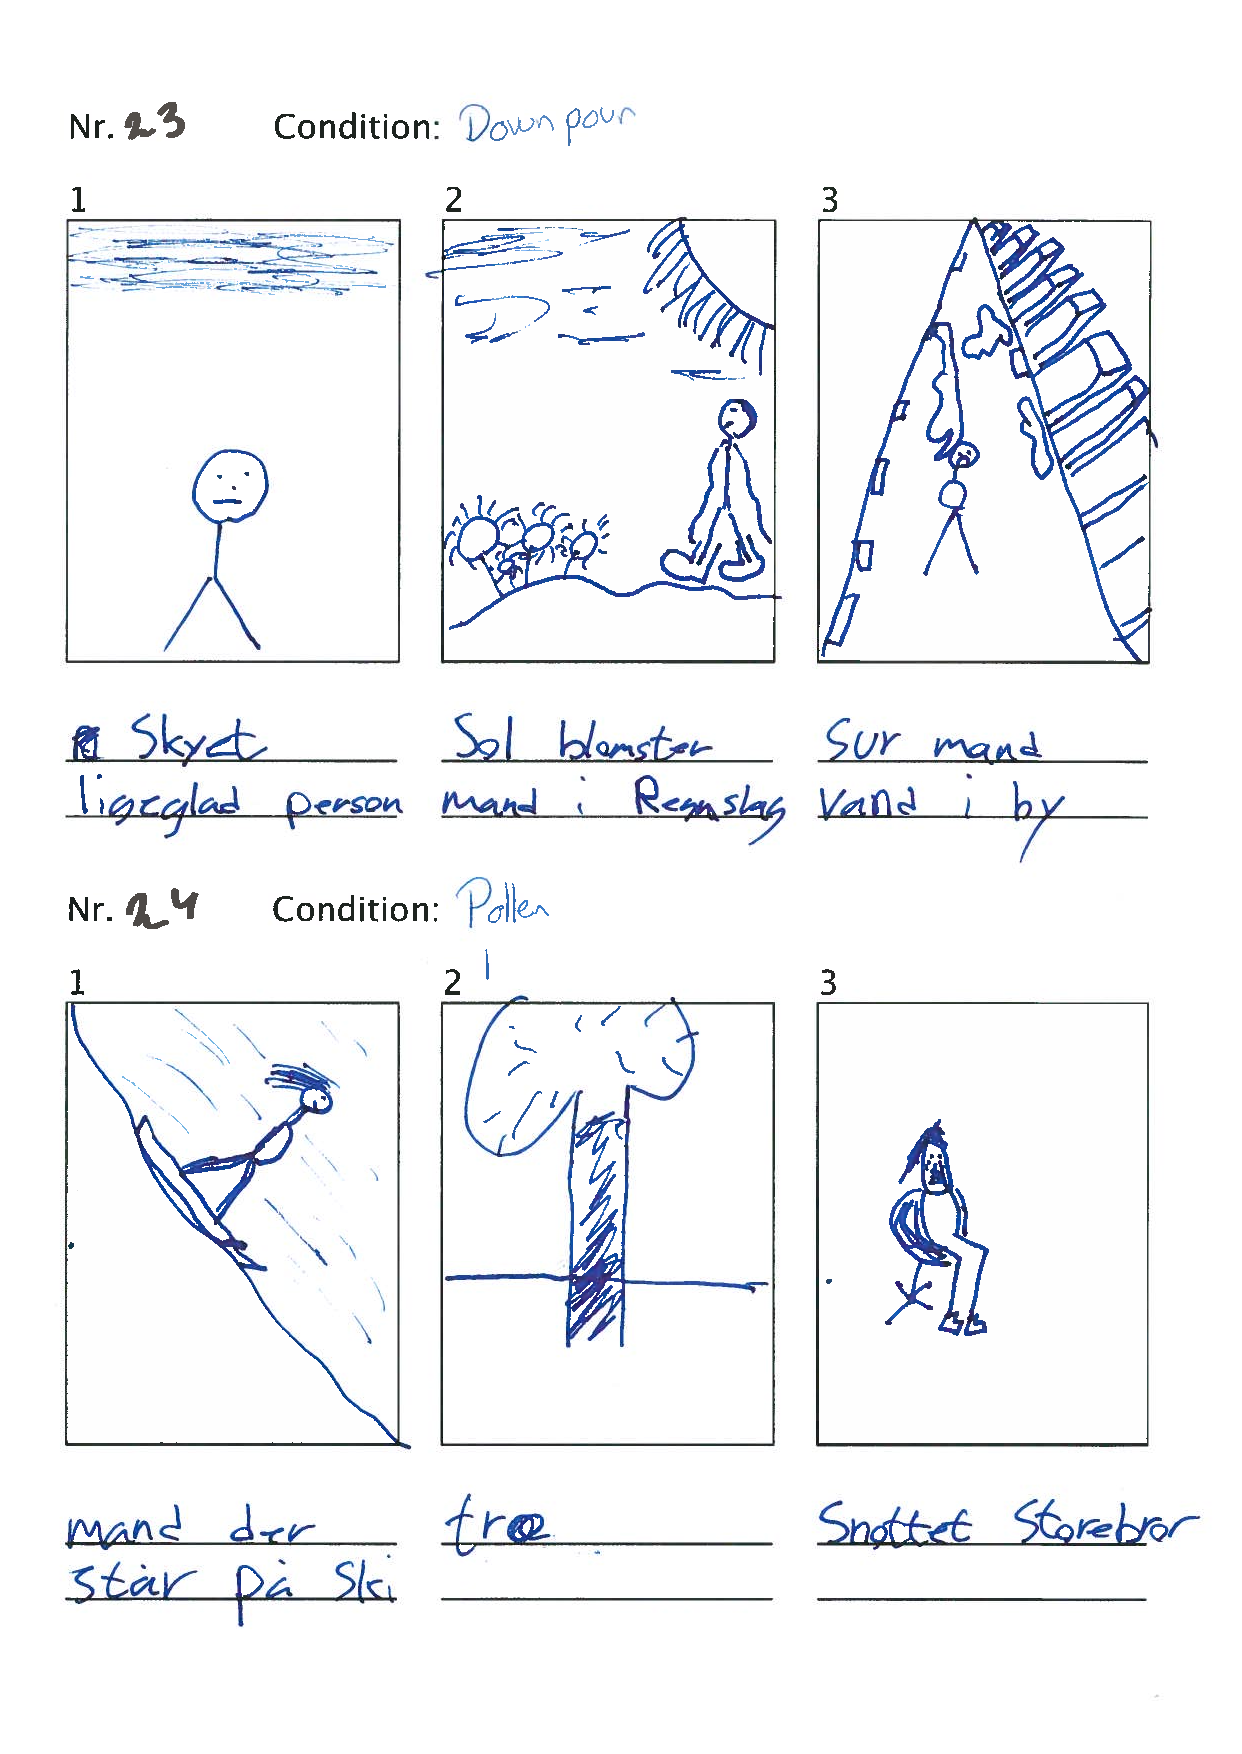
\includepdf[pages=-]{./appendices/Scan.pdf}

% subsection raw_results (end)

\subsection{Processed Results} % (fold)
\label{sub:processed_results}

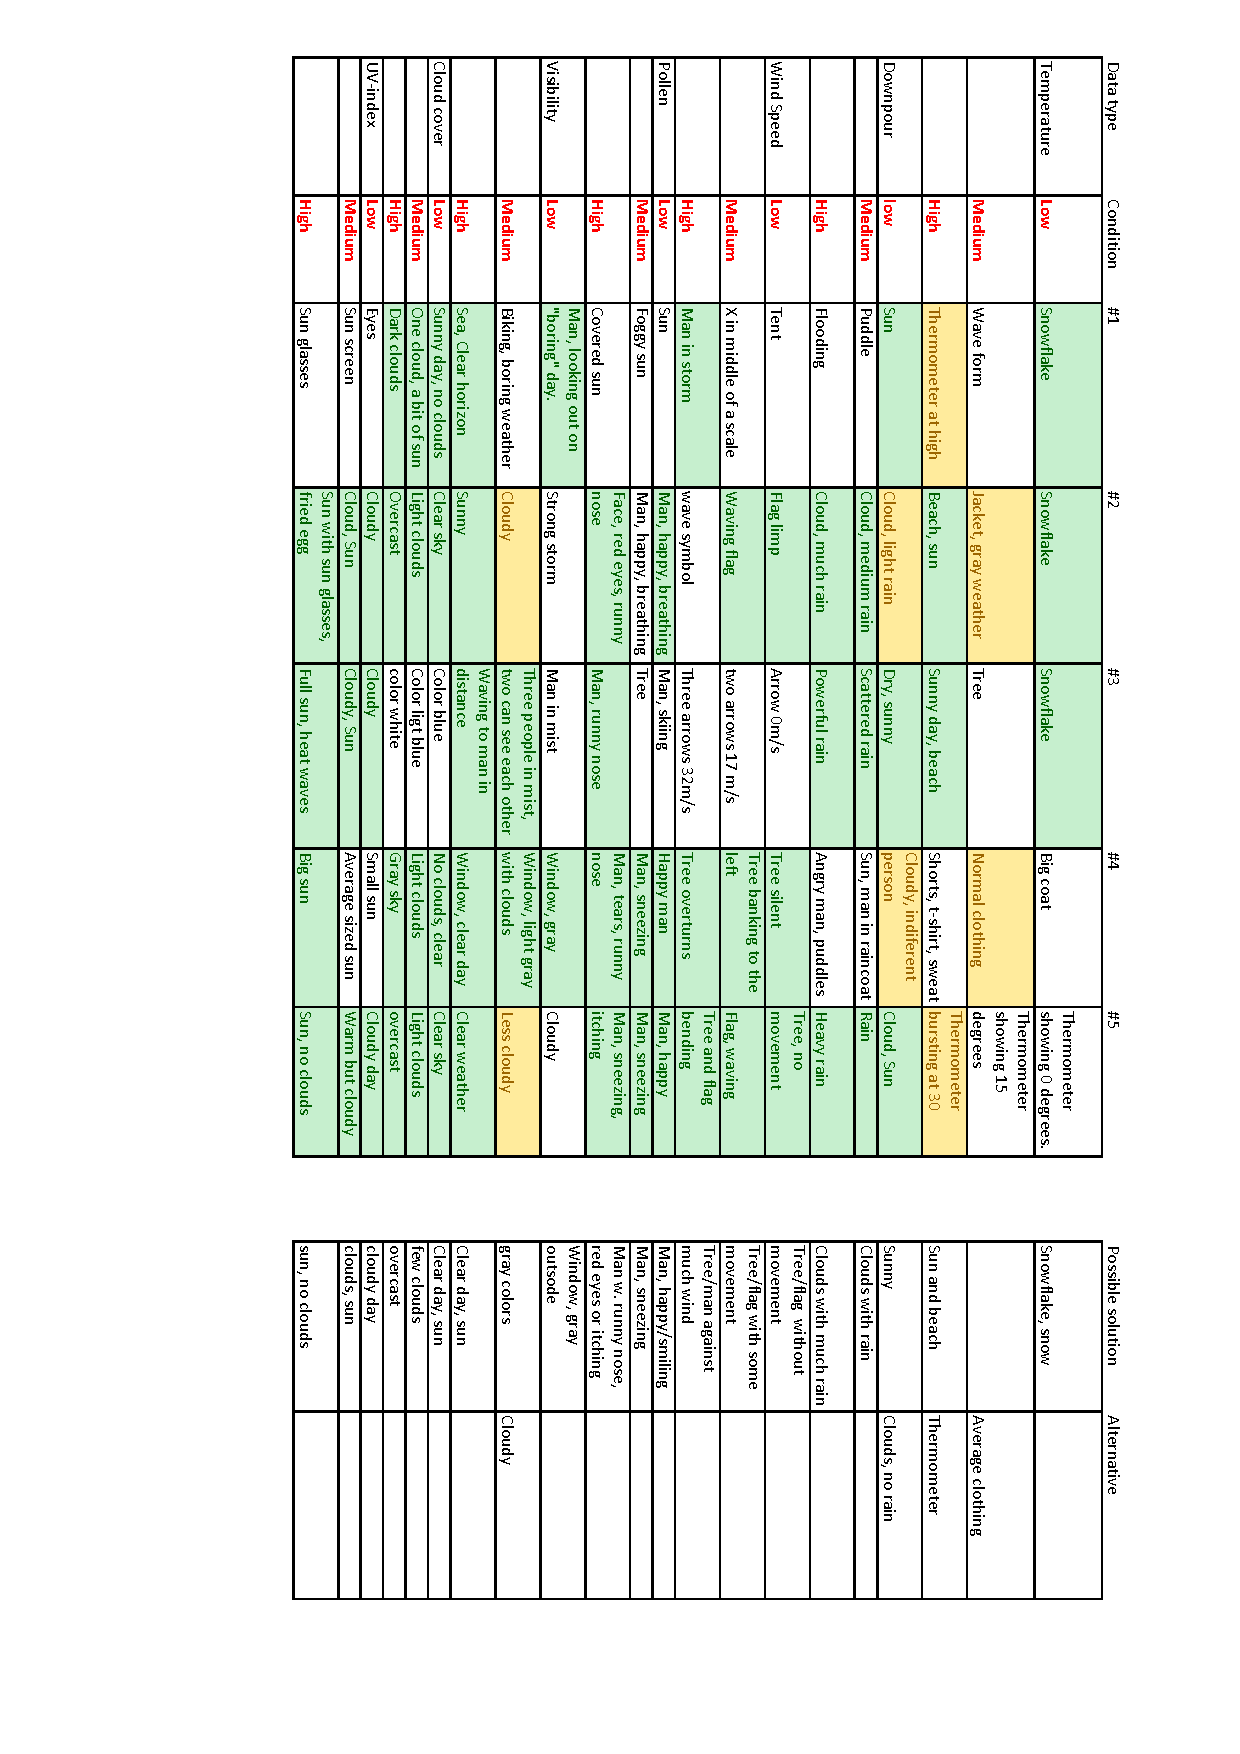
\includepdf{./appendices/Ark1.pdf}

% subsection processed_results (end)


\section{Auditory Pre-test} % (fold)
\label{sec:auditory_pre_test}
\subsection{Pre-test 1 results} % (fold)
\label{sub:pre_test_1_results}
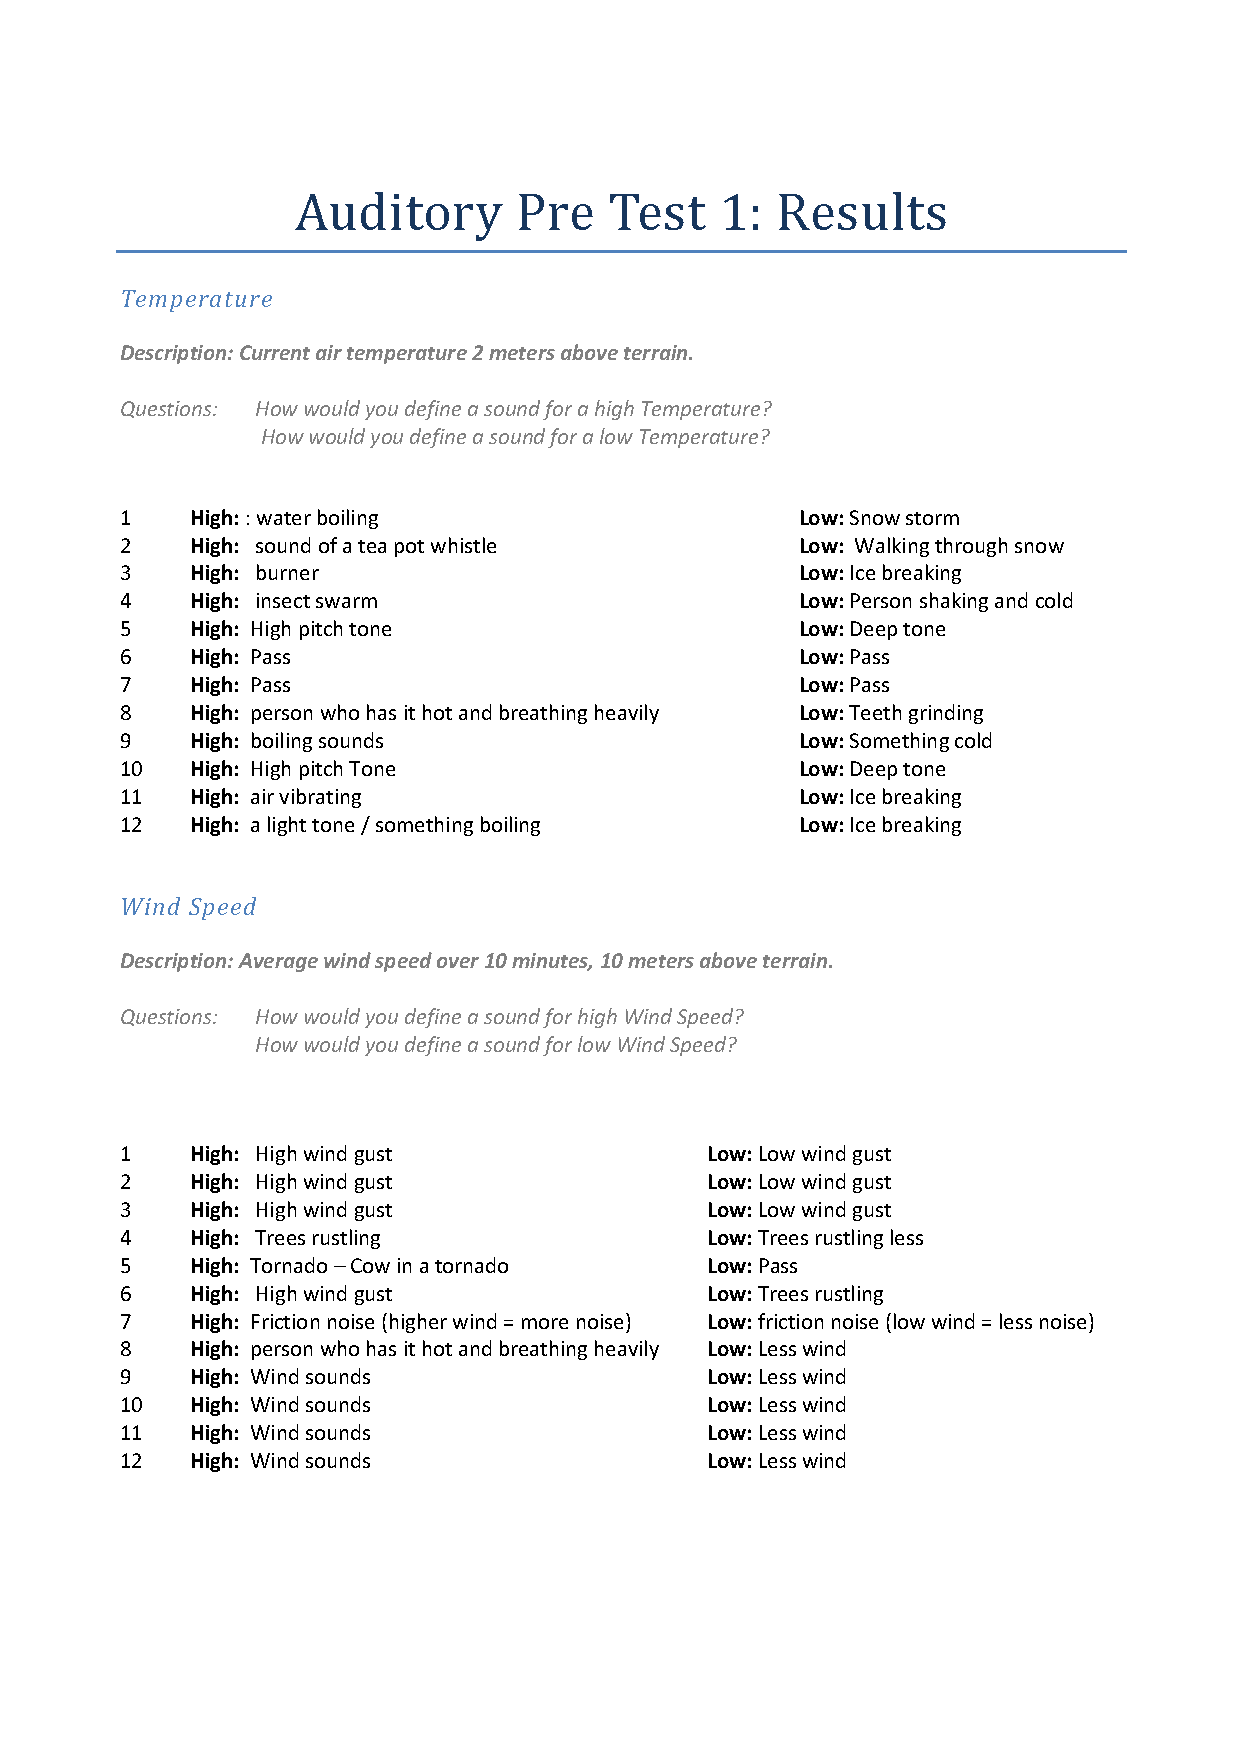
\includepdf[pages=-]{./appendices/Appendix3.pdf}
% subsection pre_test_1_results (end)

\subsection{Pre-test 2 results} % (fold)
\label{sub:pre_test_2_results}
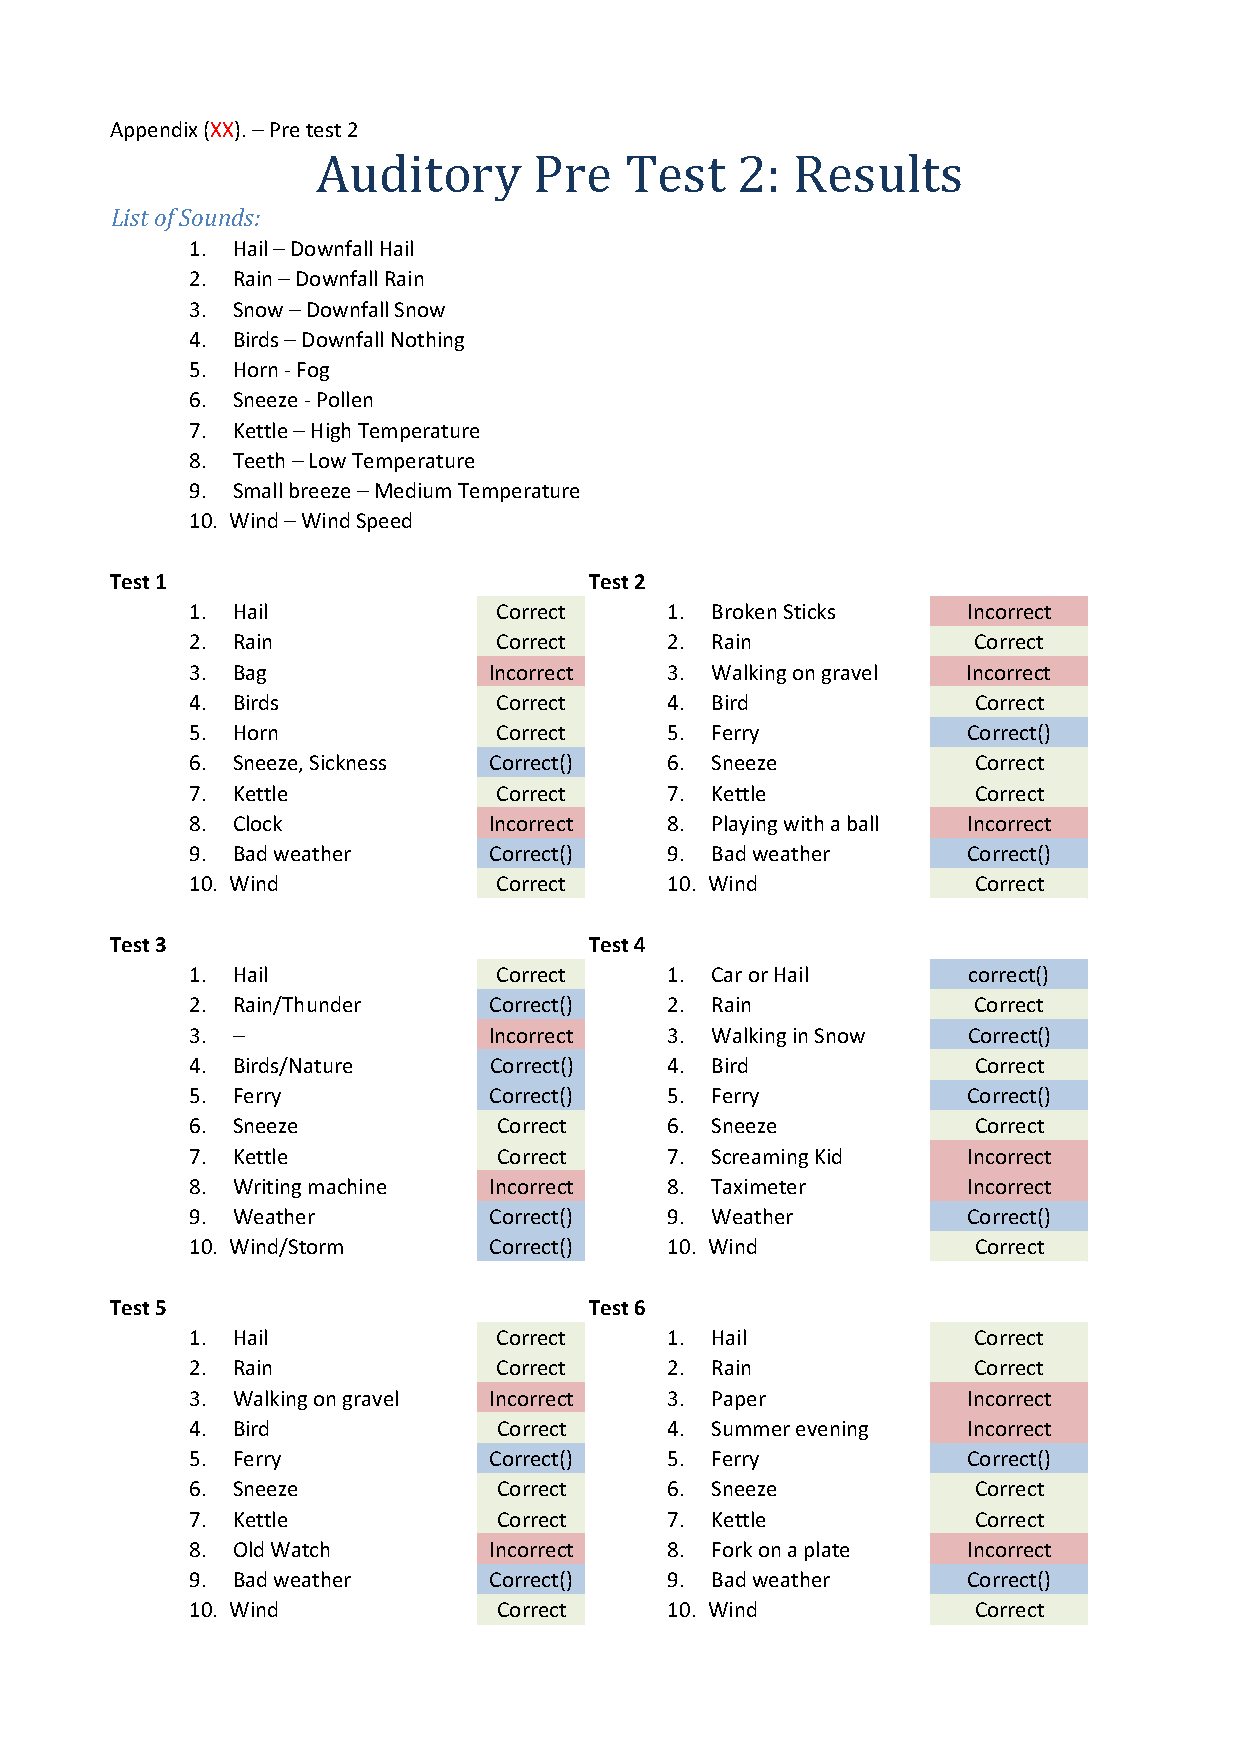
\includepdf[pages=-]{./appendices/pretest2.pdf}
% subsection pre_test_2_results (end)

\subsection{Pre-test 3 results} % (fold)
\label{sub:pre_test_3_results}
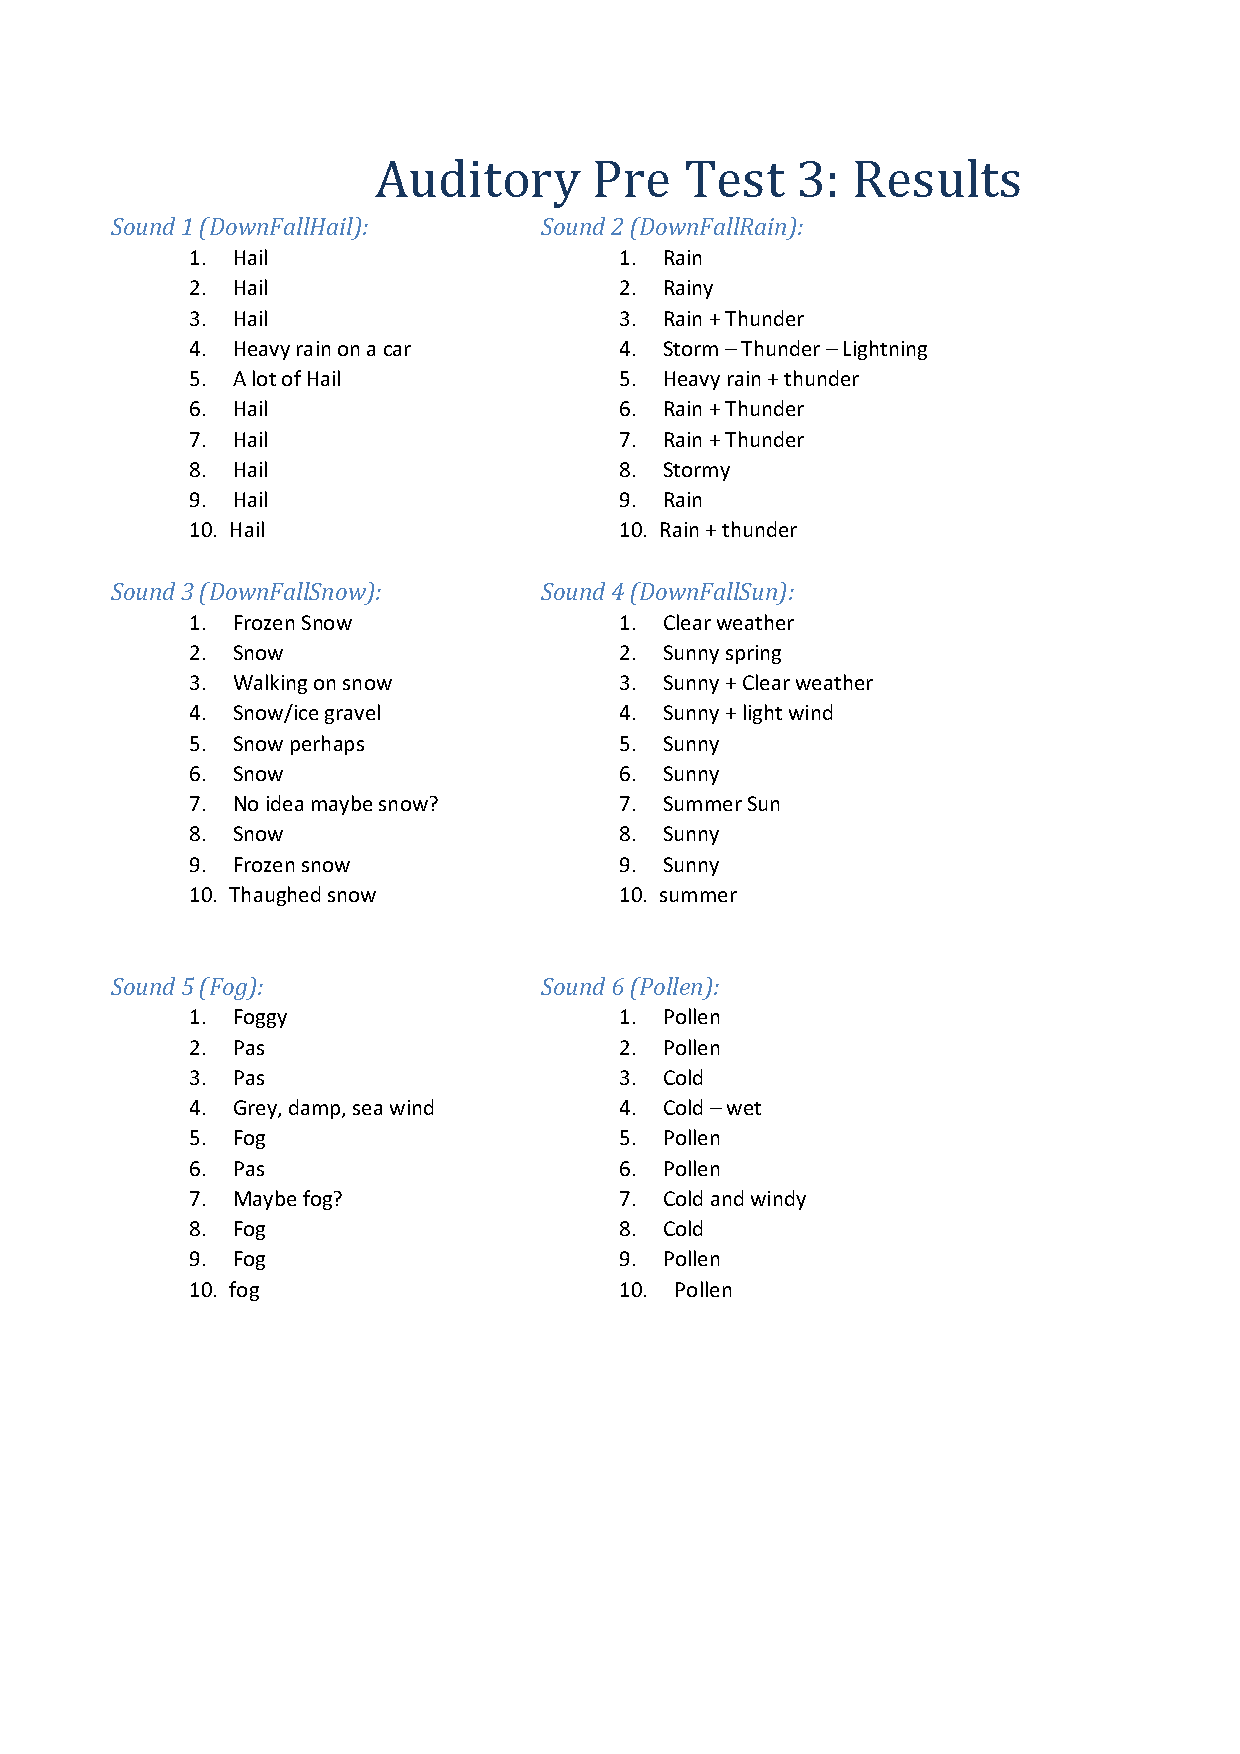
\includepdf[pages=-]{./appendices/pretest3.pdf}
% subsection pre_test_3_results (end)

% section auditory_pre_test (end)

\section{Evaluation Test Results} % (fold)
\label{sec:test_results}

\subsection{Test Result Data} % (fold)
\label{sub:test_result_data}
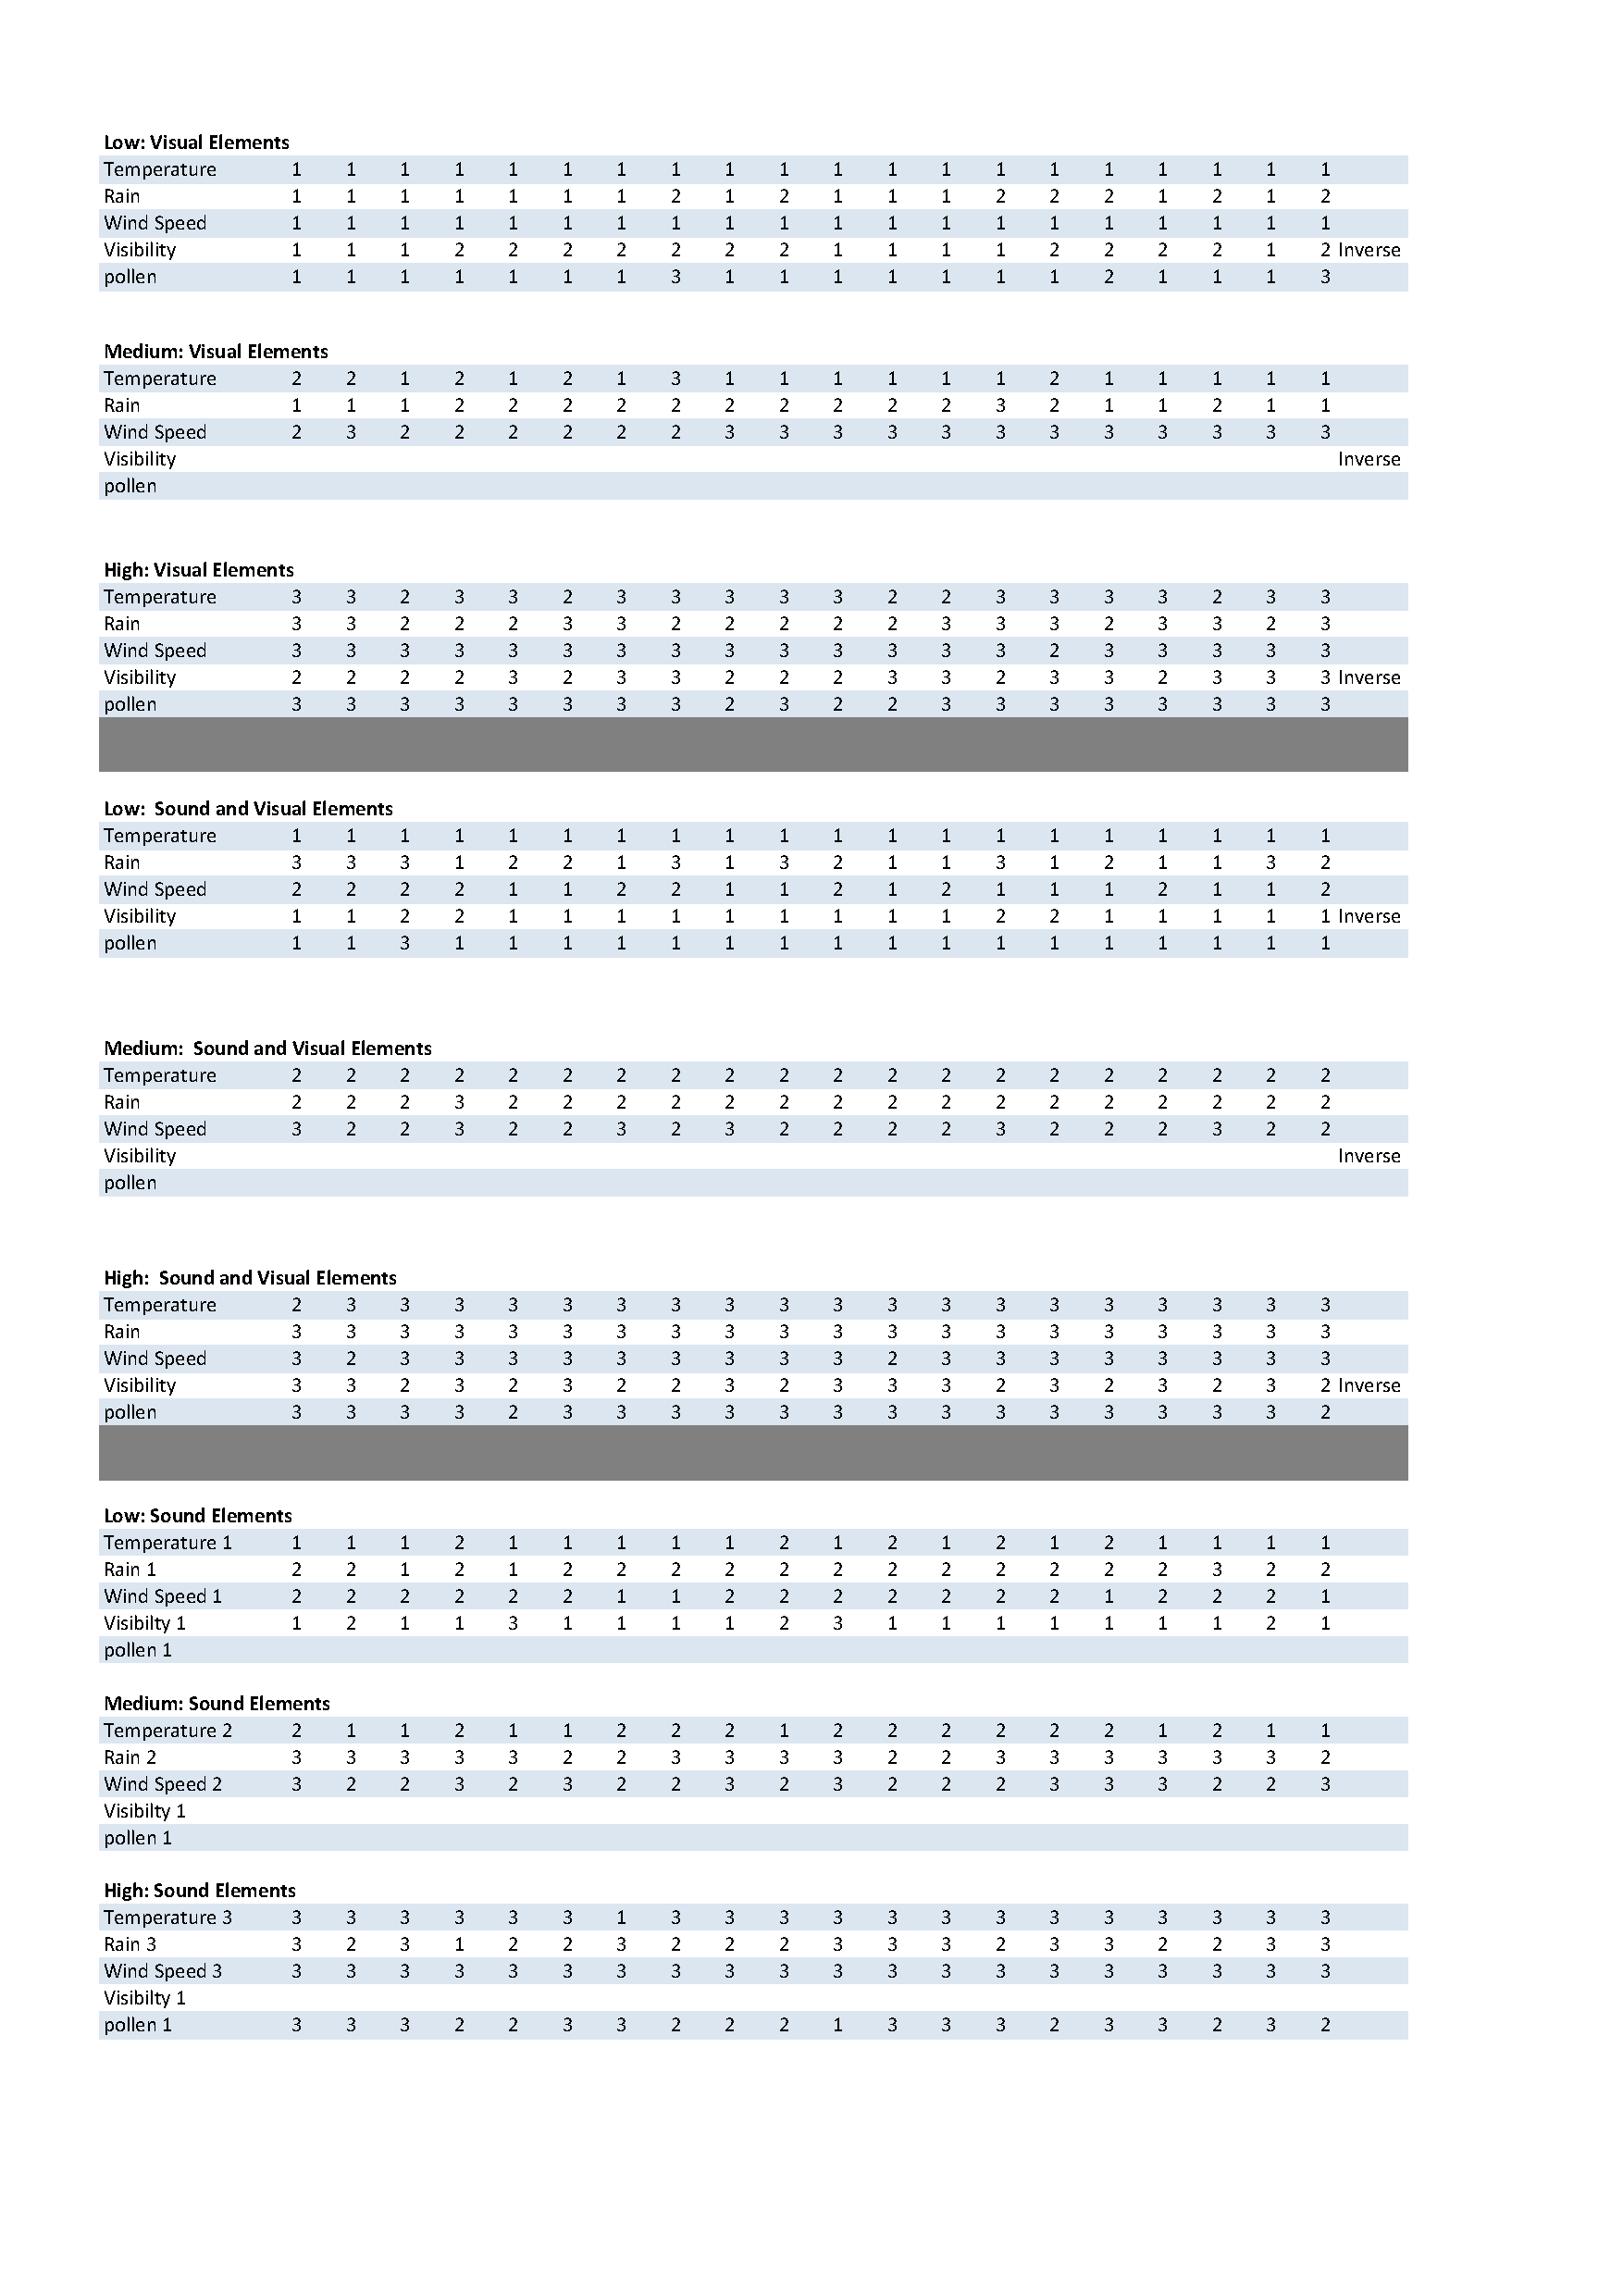
\includepdf{./appendices/Appendix6.pdf}
% subsection test_result_data (end)

\subsection{Test Result Graphs} % (fold)
\label{sub:test_result_graphs}
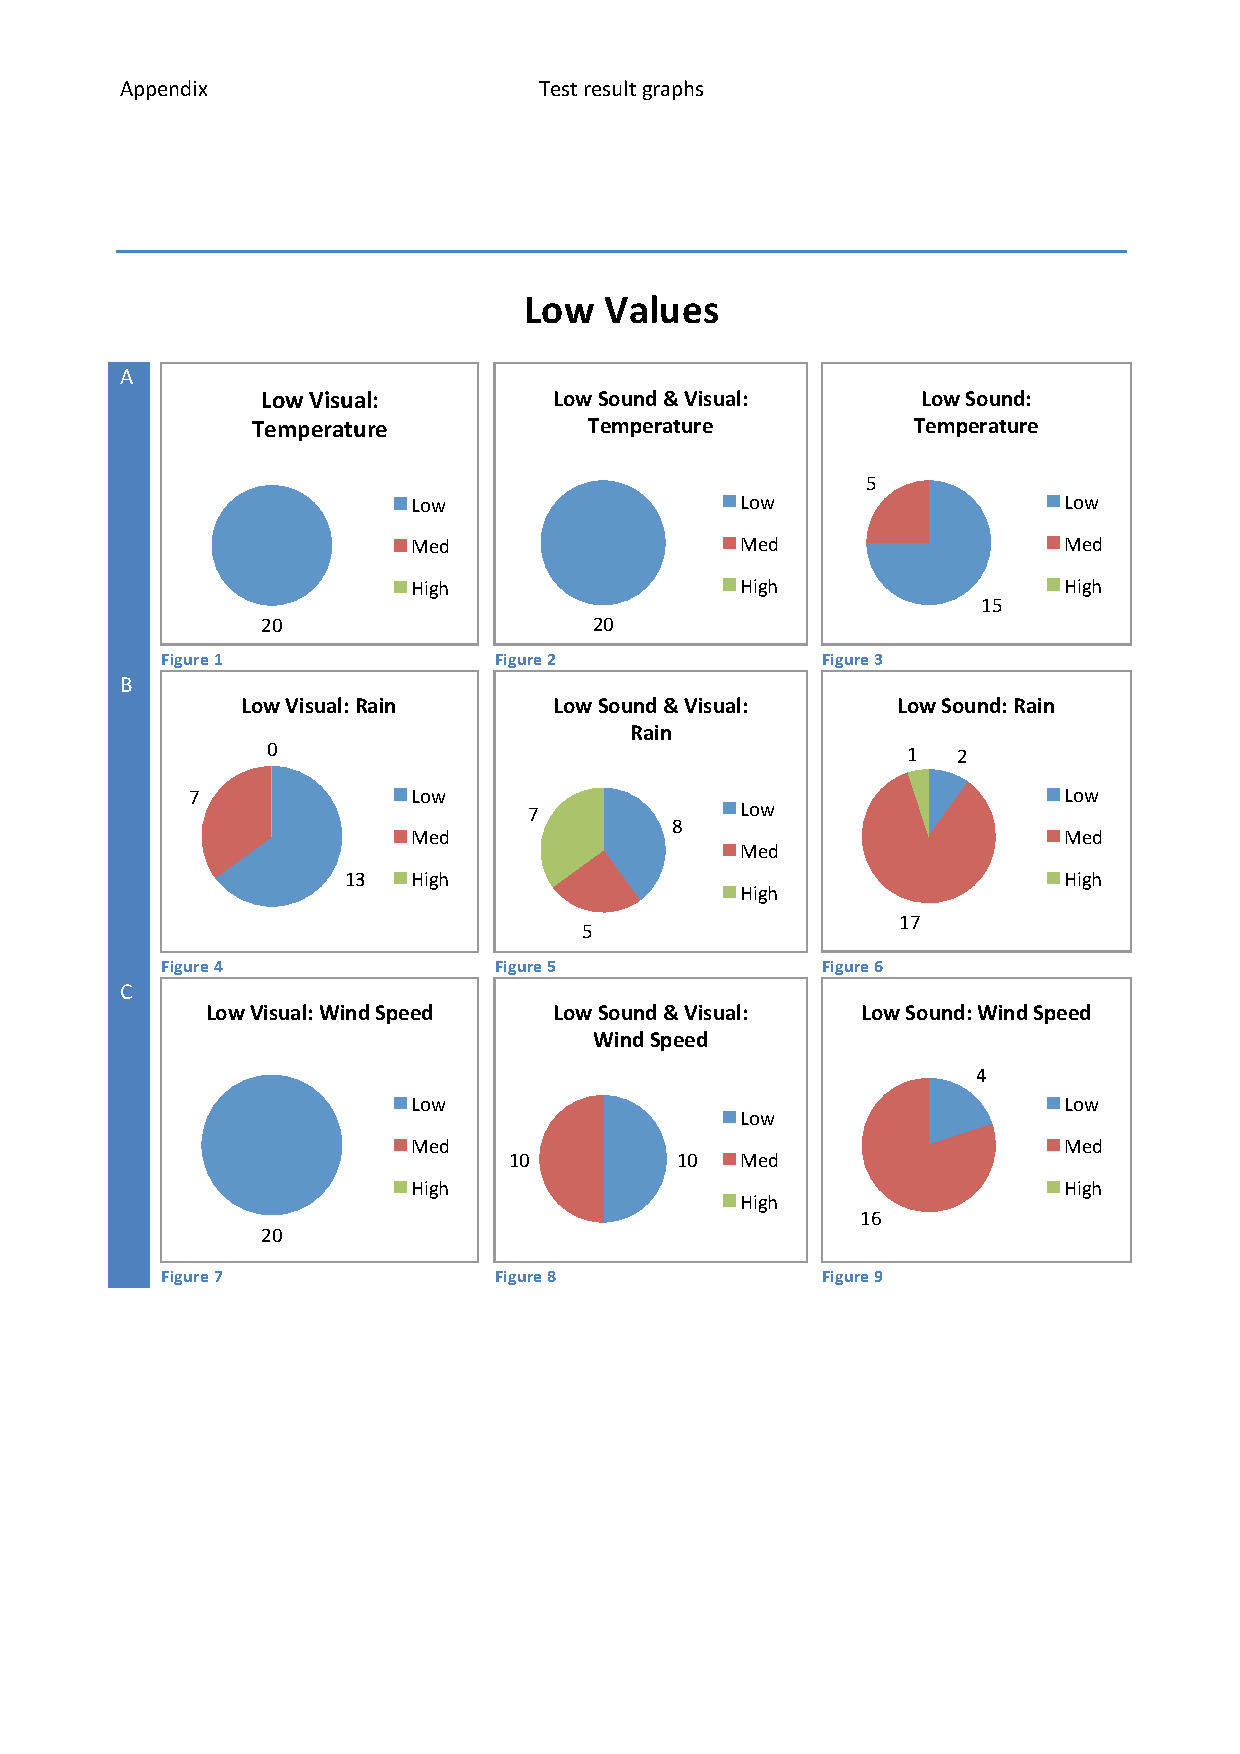
\includepdf[pages=-]{./appendices/Appendix7.pdf}
% subsection test_result_graphs (end)

% section test_results (end)

\end{document}
